\documentclass[11pt,a4paper]{article}
\usepackage[utf8]{inputenc}
\usepackage[german]{babel}
\usepackage[T1]{fontenc}
\usepackage{amsmath}
\usepackage{amsfonts}
\usepackage{amssymb}
\usepackage{graphicx}
\usepackage[margin=1.25cm]{geometry} % Puts the same margin on all borders of the document

% Packages

\usepackage{hyperref} % Generate hyperlinks to referenced items
\usepackage{adjustbox} % Used to change parameters in \includegraphics[scale=•]{•}
\usepackage{enumitem} % Provides several options for lists
\usepackage{verbatim} % Package to use \begin{comment}
\usepackage{pdfpages} % Used to import PDF pages
\usepackage{multirow} % Allows us to have a single cell in a table span multiple rows
\usepackage{makecell} % Allows us to format multiple lines in a single cell
\usepackage{listings} % Used to type code in \begin{lstlisting}
\usepackage{xcolor}  % Gives access to coloring text
\usepackage{longtable} % Allows us to create a table over multiple pages
\usepackage{float} % Improved placement of floating items
\usepackage{pdfpages} % Used to import pdf pages
\usepackage{booktabs} % Used for horizontal lines instead of \hline



% Settings

\graphicspath{{./files/}} % Sets path for files to the files folder in the same directory

\hypersetup{
    colorlinks=false, %set true if you want colored links
    linktoc=all,     %set to all if you want both sections and subsections linked
    linkcolor=blue,  %choose some color if you want links to stand out
}


\begin{titlepage}
  \title{AUD Reference Sheet} % document_name-type_of_document
  \author{Frederick Wichert}
  \date{Last Edited: \today}
\end{titlepage}


\begin{document}
	\pagenumbering{gobble}
	\maketitle
	
	\setcounter{secnumdepth}{2}
	\setcounter{tocdepth}{2}
	\tableofcontents
	
	\newpage
	\pagenumbering{arabic}



\section{Begriffsdefinitonen}
	\subsection{Allgemein}
		\begin{table}[H]
			\begin{tabular}{ p{4cm} p{13.5cm} }
				\hline
				\makecell[l]{Problem} &
				\makecell[l]
				{
					\begin{minipage}{13.5cm}
						\paragraph{} \mbox{} \\ 
						Ein Problem im Sinner der Informatik enthält eine Beschreibung der Eingabe,
						der Ausgabe, aber keinen Übergang. Eine \textbf{Probleminstanz} eine bestimmte
						Belegung der Eingabevariablen
					\end{minipage}
				} \\ \hline		

				\makecell[l]{Algorithums} &
				\makecell[l]
				{
					\begin{minipage}{13.5cm}
						\paragraph{} \mbox{} \\
						Ein Algorithmus ist eine endliche Folge von Rechenschritten, die eine Eingabe
						in eine Ausgabe umwandelt.
					\end{minipage}
				} \\ \hline

				\makecell[l]{Datenstruktur} &
				\makecell[l]
				{
					\begin{minipage}{13.5cm}
						\paragraph{} \mbox{} \\
						Eine Datenstruktur ist eine Methode, Daten abzuspeichern und zu organisieren, 
						sowie deren Zugriff auf die Daten und die Modifikation der Daten zu erleichtern.
					\end{minipage}
				} \\ \hline
			\end{tabular}
		\end{table}


\newpage
\section{Algorithmen}
	\subsection{Definition}
		Ein Algorithmus ist eine endliche Folge von Rechenschritten, die eine \textbf{Eingabe} in eine \textbf{Ausgabe} umwandelt.


	\subsection{Anforderungen}
		$\rightarrow$ Spezifizirung der Eingabe und Ausgabe \\
		$\rightarrow$ Eindeutigkeit - Jeder Einzelschritt ist klar definiert mit festgelgeter Reihenfolge \\
		$\rightarrow$ Endlichkeit - Die Notation hat eine Endliche Länge


	\subsection{Eigenschaften}
		$\rightarrow$ Determiniertheit - Für gleiche Eingabe wird gleiche Ausgabe berechnet (mögliche, andere Zwischenzustände) \\
		$\rightarrow$ Determinismus - Für die gleiche Eingabe ist die Ausführung und Ausgabe identisch \\
		$\rightarrow$ Terminierung - Der Algorithmus läuft für jede Eingabe nur endlich lange \\
		$\rightarrow$ Korrektheit - Der Algorithmus berechnet stets die spezifizierte Ausgabe, falls dieser terminiert \\
		$\rightarrow$ Effzienz - Sparsamkeit bei Ressourcen (Zeit, Speicher, Energie etc.)


	\subsection{Effizienz von Algorithmen}
		\begin{itemize}
			\item Effizienzfaktoren
			\begin{itemize}
				\item Rechenzeit (Anzahl der Einzelschritte)
				\item Kommunikationsaufwand (z.B. Netzwerk)
				\item Speciherplatzbedarf 
				\item Zugriff auf Speicher (z.B. Festplatte) \\
			\end{itemize}
			\item  (Konkret) Laufzeit hängt von vielen Faktoren ab
			\begin{itemize}
				\item Länge der Eingabe 
				\item Implementierung der Basisoperationen
				\item Takt der CPU
			\end{itemize}
		\end{itemize}


	\subsection{Divide-and-Conquer}
		\begin{itemize}
			\item \textbf{Prinziep:} \\
				Zerlege das Problem und löse es direkt \textit{oder} durch weitere Zerlegung
			\item \textbf{Divide:} \\
				Teile das Problem un mehrere Teilprobleme auf, die kleinere Instanzen des gleichen Problems darstellen
			\item \textbf{Conquer:} \\
				Beherrsche die Teilprobleme rekursiv. Wenn die Teilprobleme klein genug sind, dann löse die Teilprobleme direkt
			\item \textbf{Combine:} \\
				Vereinige die Lösungen der Teilprobleme zur Lösung des ursprünglichen Problems
		\end{itemize}


\newpage
\section{Asymptotische Komplexität}
	\subsection{Allgemein}
		Eine Abschätzung des (zetilichen) Aufwands eines Algorithmus in Abhängigkeit der Eingabe
		in form einer Asymptote in Abhängigkeit der Eingabemenge $n$.

		\begin{itemize}
			\item Beispiel: Summe bis n
			\begin{itemize}
				\item \texttt{summe=summe+i}
				\item Ablauf:
				\begin{itemize}
					\item Variablen deklarieren
					\item 1 zur Summe addieren
					\item 2 zur Summer addieren
					\item \dots
					\item n zur Sumer addieren
					\item Ausgabe der Summe
				\end{itemize}
				\item Alle Basisoperationen benötigen konstant viel Aufwand 
				\item Anzahle der Operationen wächst mit Eingabe n
				\item Für liner wachsende Eingabe wächst der Aufwand auch linear
			\end{itemize}
			\item Beispiel: Laufzeit von InsertionSort
			\begin{itemize}
				\item Quadratische Funktion: $an^2 + bn + c$
				\item Bei gro\ss em n überweigt der quadratische Anteil $\rightarrow$ Terme niedriger Ordnung werden irrelevant
				\item s
			\end{itemize}
		\end{itemize}


	\subsection{Asymptotische Notation}
		\begin{itemize}
			\item Wie ist das Verhalten der Laufzeit $T(n)$ für sehr gro\ss e Eingaben $  \in N$
			\begin{itemize}
				\item bei kleinen Eingaben (z.B. $n = 5$) ist die reale Laufzeit mehr dominiert 
					von den Initialisierungskosten und nicht dem Algorithmus selbst
					\item Komplexität ist unabhängig von konstanten Faktoren und Summanden
				\item Berücksichtigen nicht Betrachtung:
				\begin{itemize}
					\item Rechnergeschwindigkeit
					\item Aufwände der Initialisierung
				\end{itemize}
				\item Komplexitätsmessungen via Funktionsklassen ausreichend
				\begin{itemize}
					\item Wie verhält sich der Algorithmus für gro\ss e Problemgrö\ss en
					\item Wie verändert sich die Laufzeit, wenn die Problemgrö\ss e verdoppelt wird
				\end{itemize}
			\end{itemize}
		\end{itemize}

		\subsubsection{Komplexitätsfunktion}
			Das Wachstumsverhalten reicht aus um die wichtigen Punkte eines Algorithmus zu veranschaulichen.

	\subsection{Schranken der asymptotischen Komplexität}
		\begin{minipage}[t]{0.32\textwidth}
			\subsubsection{Best case}
				\begin{itemize}
					\item Komplexität im "besten" Fall
					\item Wie schnell ist der Algorithmus, wenn der Input so vorliegt, dass dieser am schnellsten terminiert?
					\item Beispiel: Vorsortierte Liste für (simplen) Sortieralgorithmus
				\end{itemize}
		\end{minipage}
		\begin{minipage}[t]{0.32\textwidth}
					\subsubsection{Average case}
						\begin{itemize}
							\item Komplexität im "durchschnittlichen" Fall
							\item Wie schnell ist der Algorithmus, wenn ein üblicher Input vorliegt?
							\item Beispiel: Zufällig verteilte Liste für (simplen) Sortieralgorithmus
						\end{itemize}
		\end{minipage}
		\begin{minipage}[t]{0.32\textwidth}
			\subsubsection{Worst case}
				\begin{itemize}
					\item Komplexität im "schlechtesten" Fall
					\item Wie schnell ist der Algorithmus, wenn der Input so vorliegt, dass dieser am spätestens terminiert?
					\item Beispiel: Negativ-sortierte Liste für (simplen) Sortieralgorithmus
				\end{itemize}
		\end{minipage}


	\subsection{Notationen und Definition}
		\subsubsection{$\Theta$-Notation}
			\begin{center}
				Funktionen $f, g: \mathbb{N} \rightarrow \mathbb{R}_{>0}$ \\
			\end{center}
			Dabei ist $\mathbb{N}$ Die Eingabelänge und $\mathbb{R}$ die Zeit 
			\begin{center}
				$\Theta(g) = \{f: \exists c_1 , c_2 \in \mathbb{R}_{>0}, n_0 , \in \mathbb{N}, \forall n \geq n_0 , 0 \leq c_1	 g(n) \leq f(n) \leq c_2 g(n)\}$
			\end{center}
			Schreibweise: $f \in \Theta (g)$ oder $f = \Theta (g)$

		\subsubsection{O-Notation - Laufzeit}
			Obere asymptotische Schranke - auch "Laufzeit" eines Algorithmus genannt
			\begin{center}
				$O(g) = \{f: \exists c \in \mathbb{R}_{>0}, n_0 , \in \mathbb{N}, \forall n \geq n_0 , 0 \leq f(n) \leq c g(n)\}$
			\end{center}
			Sprechweise: $f$ wächst höchstens so schnell wie g \\
			Sprechewise: $f = O(G)$ \\\\

			\noindent Beachte: $f(n) = \Theta (n) \implies f(n) = O(n)$ \\
			\indent \hspace{1.5cm} $\Theta (g(n)) \subseteq O(g(n))$ \\

			\noindent Rechenregeln
			\begin{itemize}
				\item Konstanten: $f(n) = a$ mit $a \in \mathbb{R}$ konstante Funktion. Dann $f(n) = O(1)$
				\item Skalare Multiplikation: $f = O(g)$ und $a \in \mathbb{R}$. Dann $a*f = O(g)$
				\item Addition: $f_1 = O(g_1)$ und $f_2 = O(g_2)$. dann $f_1 + f_2 = O(max\{ g_1, g_2\})$
				\item Multiplikation: $f_1 = O(g_1)$ und $f_2 = O(g_2)$. dann $f_1 * f_2 = O(g_1 * g_2)$
			\end{itemize}

		\subsubsection{$\Omega$-Notation}
			Untere asymptotische Schranke
			\begin{center}
				$\Omega(g) = \{f: \exists c \in \mathbb{R}_{>0}, n_0 , \in \mathbb{N}, \forall n \geq n_0 , 0 \leq c g(n) \leq f(n)\}$
			\end{center}
			Sprechweise: $f$ wächst mindestens so schnell wie g \\
			Sprechewise: $f = \Omega(G)$ \\

			\begin{center}
				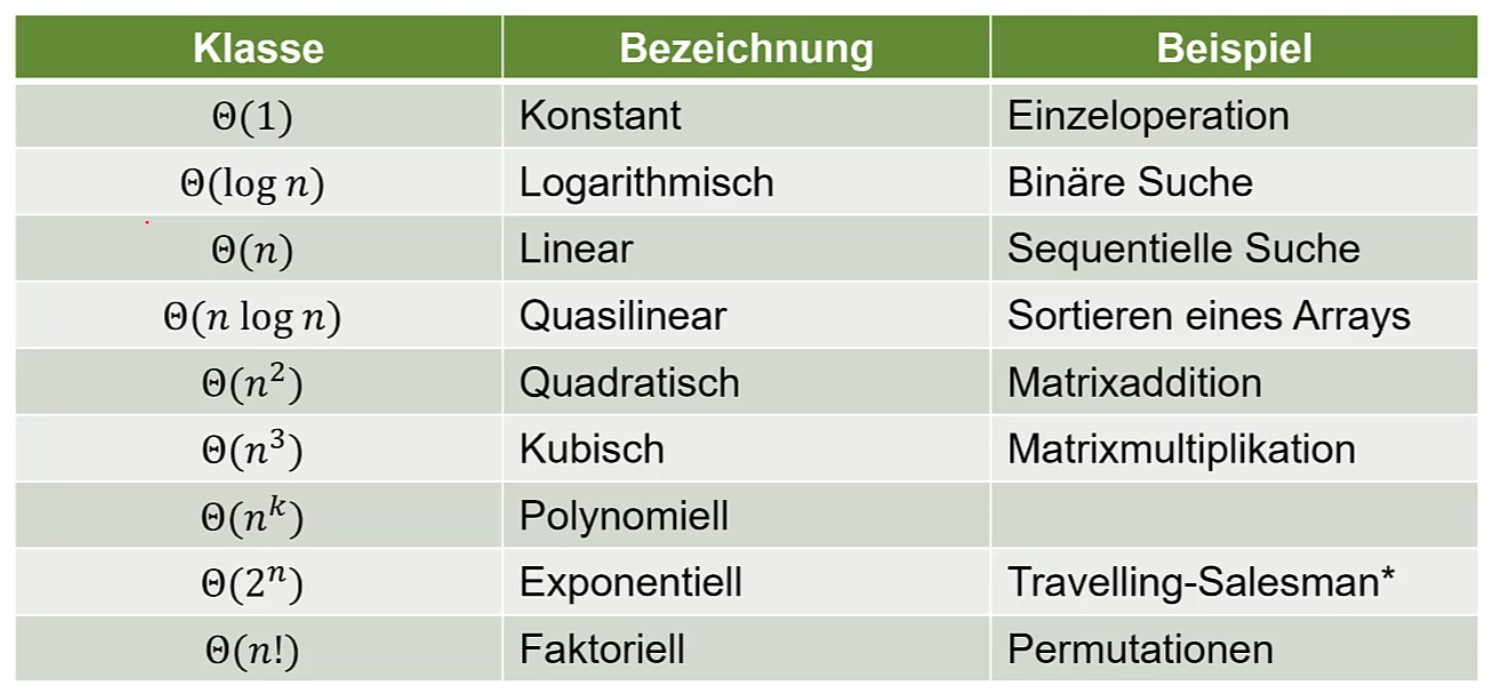
\includegraphics[scale=0.4]{Notation_Exsample.jpg}
			\end{center}


		\subsubsection{$\theta$ und $\omega$}
			TODO



\newpage
\section{Analyse von Divide-and-Conquer Algorithmen}
	\subsection{Allgemein}
		$T(n)$ ist Laufzeit eines Problems der Grö\ss e $n$. \\ \\
		\noindent Für kleines Problem, d.h. $n \leq c$ mit $c$ ist eine Konstante, dann benötigt 
		die Direkte Lösung konstante Zeit $\Theta (1)$. \\ \\
		\noindent Für sonstige $n$ gilt: Das Aufteilen des Problems führt zu $a$ Teilproblemen, 
		von denen jedes die grö\ss e 1/$b$ der Grö\ss e des ursprünglichen Problems hat. \\ \\
		\noindent Das Lösen eines Teilproblems der Grö\ss e $n$/$b$ dauert $T(n/b)$ und somit 
		benötigen wir für das Lösen von $a$ solcher Probleme $aT(n/b)$. \\ \\
		\noindent $D(n)$ ist die Zeit um das Problem aufzuteilen, $C(n)$ ist die Zeit um die 
		Teillösungen zur Lösung des ursprünglichen Problems zusammenzufügen. \\

		\begin{center}
			\[
				T(n) = \left\{\begin{array}{lr}
					\Theta (1) & \\
					aT(n/b) + D(n) + C(n) &
					\end{array}\right\}
			\] \\
			Falls $n \leq c$ \vspace{1cm}
		\end{center}


	\subsection{Methoden zur Lösung von Rekursionsgleichung}
		\noindent \textbf{Substitutionsmethode:} wir erraten eine Schranke und nutzen methematische Induktion, 
		um die Korrektheit zu beweisen.

		\noindent \textbf{Rekursionsbaum-Methode:} wandelt die Rekursionsgleichung in einen Baum um, 
		dessen Knoten die Kosten der Rekursion in den versxchiedenen Ebenen darstellt.

		\noindent \textbf{Mastermethode:} leifert Schranken für Rekursionsgleichung der Form: $T(n) = aT(n/b) + f(n)$


		\subsubsection{Substitutionsmethode}
			Zur Lösung der Rekursionsgleichung, 2 Schritte:
			\begin{itemize}
				\item Rate die Form der Lösung, z.B. durch 
				\begin{itemize}
					\item Scharfes Hinsehen
					\item kurze Eingaben ausprobieren und einsetzen
				\end{itemize}
				\item Anwendung von vollständiger Induktion, um die Konstante zu finden und zu zeigen, dass
				das Geratene eien Lösung ist
			\end{itemize}


		\subsubsection{Rekursionsbaum-Methode}
			Grundidee: Stelle das Ineinander-Einsetzen als Baum dar und analysiere die Kosten
			\begin{enumerate}
				\item Jeder Knoten stellt die Kosten eines Teilproblems dar.
				\begin{itemize}
					\item Die Wurzel stellt die zu analysierenden Kosten $T(n)$ dar
					\item Die Blätter stellen die Kosten der Basisfälle dar, z.B. $T(0)$
				\end{itemize}
				\item Berechnen die Kosten innerhalb jeder Ebene des Baums
				\item Die Gesamtkosten ist die Summe über die Kosten aller Ebenen
			\end{enumerate}
			Geratenes kann durch Substitutionsmethode überprüft werden.


		\subsubsection{Mastermethode}
			Allgemeine Form der Rekursionsgleichung: \\
			\noindent $T(n) = aT(n/b) + f(n)$ mit $q \geq 1, b > 1$ und $f(n)$ eine asymptotische positive Funktion.

			\begin{itemize}
				\item Problem wird in $a$ Teilprobleme der grö\ss e $n/b$ aufgeteilt.
				\item Lösen jedes der $a$ Teilprobleme benötigt Zeit $T(n/b)$.
				\item Funktion $f(n)$ umfasst die Kosten, um das Problem in Teilprobleme aufzuteilen
					und um die Teillösungen zu vereinigen.
			\end{itemize}

	\subsection{Mastertheorem}
			Seien $a \geq 1$ und $b > 1$ Konstanten. Sei $f(n)$ eine positive Funktion und $T(n)$
			über den nicht negativen ganzen Zahlen durch die Rekursionsgleichung
			\begin{center}
				$T(n) = aT(n/b) + f(n)$
			\end{center}
			definiert, wobei wir $n/b$ so interpretieren, dass damit entweder $\lfloor n / b \rfloor$
			oder $\lceil n/b \rceil$ gemeint ist. Dann besitzt $T(n)$ die folgenden asymptotischen Schranken:
			\begin{enumerate}
				\item Gilt $f(n) = O(n^{\log_b a-\epsilon})$ für eine Konstante $\epsilon > 0$, dann $T(n) = \Theta (n^{\log_b a})$.
				\item Gilt $f(n) = \Theta (n^{\log_b a})$, dann gilt $T(n) = \Theta (n^{\log_b a} \lg n)$.
				\item Gilt $f(n) = \Omega (n^{\log_b a+\epsilon})$ für eine Konstante $\epsilon > 0$ und $af(n/b) \leq cf(n)$
					für eine Konstante $c < 1$ und hinreichend gro\ss en $n$, dann ist $T(n) = \Theta (f(n))$.
			\end{enumerate} 
			Das Mastertheorem verstehen: \\
			In jedem der 3 Fälle wird die Funktion $f(n)$ mit $n^{\log_b a}$ verglichen. \\
			Intuition:  
			\begin{enumerate}
				\item Wenn $f(n)$ olynomial kleiner ist als $n^{\log_b a}$, dann $T(n) = \Theta (n^{\log_b a})$.
				\item Wenn $f(n)$ und $n^{\log_b a}$ die gleiche Gr\ss e haben, dann gilt $T(n) = \Theta (n^{\log_b a} \lg n)$.
				\item Wenn $f(n)$ polinimial gr\ss er ist als $n^{\log_b a}$ und $af(n/b) \leq cf(n)$ erfüllt, dann ist $T(n) = \Theta (f(n))$.
			\end{enumerate}
			\textbf{Nicht} abedeckte Fälle sind:
			\begin{enumerate}
				\item Wenn $f(n)$ kleiner als $n^{\log_b a}$, aber nicht polinimial klainer.
				\item Wenn $f(n)$ grö\ss er als $n^{\log_b a}$, aber nicht polinimial grö\ss er.
				\item Regularitätsbedingung $af(n/b) \leq cf(n)$ nicht erfüllt.
			\end{enumerate}

\newpage
\section{Sortieralgorithmen}
	\subsection{Sortieralgorithmen: Theorie}
		\subsubsection{Warum möchte man Sortieren}
			\begin{itemize}
				\item Sachen Packen
				\item Zeitmanagement
				\item etc
			\end{itemize}
		
		
		\subsubsection{Bedingungen}
			- Ausgangspunkt als Folge von Datensätzen \\
			- Zu sortierenden elemente hei\ss en Schlüsselelemente (-werte) \\
			- Ziel: Schlüsselwerte nach einem Ordnungsschlüssel zu sortieren \\
			\textbf{Bedingug} $\rightarrow$ Schlüsselwerte müssen vergleichbar sein
		
		
		\subsubsection{Vergleichskriterien}
			- Berechnungsaufwand: O(n) \\
			- Effizienz: Best Case vs. Average Case vs. Worst Case \\ 
			- Speicherbedarf:
			$\rightarrow$ in-place: zustzlicher Speicher von der Eingabegrö\ss e unabhängig \\
			$\rightarrow$ out-of-place: Speichermerhbedarf von eingabegrö\ss e abhängig \\
			- Stabilität: Erahltenbleiben des sekundären Sortierschlüssels \\
		
			$\rhd$ Sortierverfahren abhängig von Anwendung, Unterschiedliche Zahl von Vertauschungen vs Vergleichungen 
		
		
		\subsubsection{Vergleichsverfahren}
			\subsubsection{Korrektheit mittels Schleifeninvariante}
				\begin{itemize}
					\item Eine Schleifeninvariante beschreibt was bei dem Durchlauf einer Schleife zu Beginn immer gegeben ist \\
						Damit kann die Korrektheit eines Algorithmus bewiesen werden \\
						$\rhd$ Vergleichbar mit einem Indutkionsbeweis 
					\item Eine Schleifeninvariante muss 3 Eigenschaften erfüllen:
					\begin{itemize}
						\item Initialisierung: Invariante ist vor jeder Iteration wahr
						\item Fortsetzung: Wenn die Invariante vor der Schleife wahr ist dann bleibt sie auch bis zum Beginn der nächsten Iteration wahr
					\end{itemize}
					\item Bei dem Insertionsort:
					\begin{itemize}
						\item Zu Beginn ist die Leinke Teilmenge immer sortiert
					\end{itemize}
				\end{itemize}
				\vspace{1.5cm}
		
		
	\subsection{Entwurfsprinzipien des Sortieren}
	
		$\rhd$ IsertionSort: inkrementelle Herangehenweise \\ \\
		
		\noindent $\rhd$ Divide-and-Conquer Ansatz (Teile-undBeherrsche):
		\begin{itemize}
			\item Ansatz um Sortieralgorithmus zu entwerfen
			\item Laufzeit: im schlechtesten Fall immer noch besser als InsertionSort
			\item Gibt Methoden mit welchen wir die Laufzeit einfach bestimmen können \\
		\end{itemize}
		
		\subsubsection{Devide-and-Conquer}
			\paragraph{Prinzip:} Zerlege das Problem und löse es direkt \textit{oder} durch weitere Zerlegung.
			\paragraph{Divide:} Teile das Problem in mehrere Teilprobleme auf, die kleinere Instanzen des gleichen Problems darstellen.
			\paragraph{Conquer:} Beherrsche die Teilprobleme rekursiv. Wenn die Teilprobleme klein genug sind, dann löse die Teilprobleme auf direktem Weg.
			\paragraph{Combine:} Vereinige die Lösung der Teilprobleme zur Lösung des ursprünglichen Problems.
		
			\begin{center}
				Beispiel: \underline{\nameref{MergeSort}}
			\end{center}
			\vspace{1.5cm}
		
		
	\subsection{InsertionSort} 
		\begin{minipage}[t]{0.5\textwidth}
			\subsubsection{Grundidee}
				\begin{itemize}
					\item Sortieren durch Einfügen:
					\item Die Linke Teilmenge ist Sortiert, und passend wird immer ein neues Element eingefügt 
				\end{itemize}
					
				\subsubsection{Eigenschaften}
					\begin{itemize}
						\item Stabieler Algorithmus
					\end{itemize}
		\end{minipage}
		\begin{minipage}[t]{0.45\textwidth}
			\subsubsection{Code}
				\begin{center}
					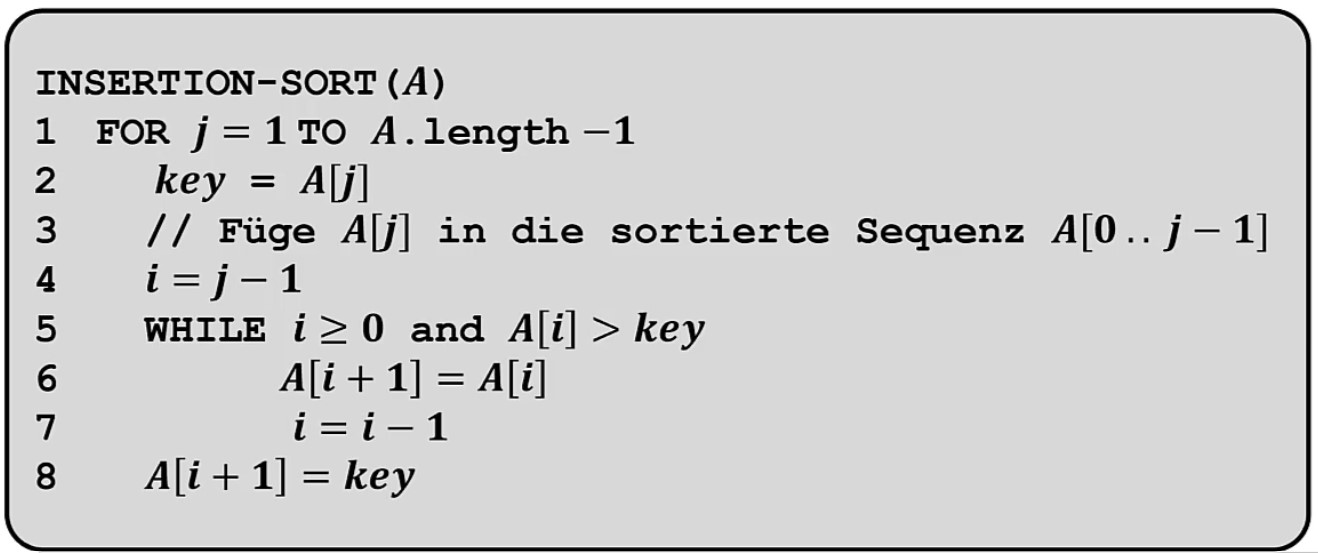
\includegraphics[scale=0.35]{InsertionSort_Code.jpg}
				\end{center}
		\end{minipage}
		\vspace{0.5cm}
		
		
		\subsubsection{Beweis der Korrektheit}
			Um die Korrekthiet des Algorithmuses zu bestimmen nutzen wir die Schleifeninvariante
			\begin{itemize}
				\item Initialisierung: Beginn mit j=1, also mit dem Teilfeld bis j-1, besteht aus einem element und ist Sortiert
				\item Fortsetzung: Zu zeigen ist, dass die Invariante bei jeder Iteration erhalten bleibt.
					Die for-Schleife verschiebt jedes Element der sortierten Menge um eins nach rechts bis das zu
					sortierende Element eingefügt werden kann. Inkrementieren von j erhält die Schleifeninvariante
				\item Terminierung: Abbruhcbedingung for-Schleife wenn j>A.length-1. Jede Itearation erhöht j.
					Dann bei Abbruch j=n und einsetzen in Invariante liefert das Teilfeld A[0...n-1] welches aus den
					ursprünglichen Elementen besteht $\rightarrow$ Teilfeld = gesamtes Feld
			\end{itemize}
			\vspace{1.5cm}
		
				
		% \subsubsection{Animation}								TODO: Animation of Algorithms
			% \begin{frame}{}
				% \animategraphics[loop,autoplay,width=\linewidth]{0.8}{InsertionSortAnim-}{0}{2}
			% \end{frame}
		
		
	\subsection{BubbleSort}
		\begin{minipage}[t]{0.5\textwidth}
			\subsubsection{Grundidee}
				$\rhd$ Vergleiche Paare von benachbarten Schlüsselwerten \\
				$\rhd$ Tausche das Paar, falls rechter Schlüsselwert kleiner ist als linker
		\end{minipage}
		\begin{minipage}[t]{0.45\textwidth}
			\subsubsection{Code}
				\begin{center}
					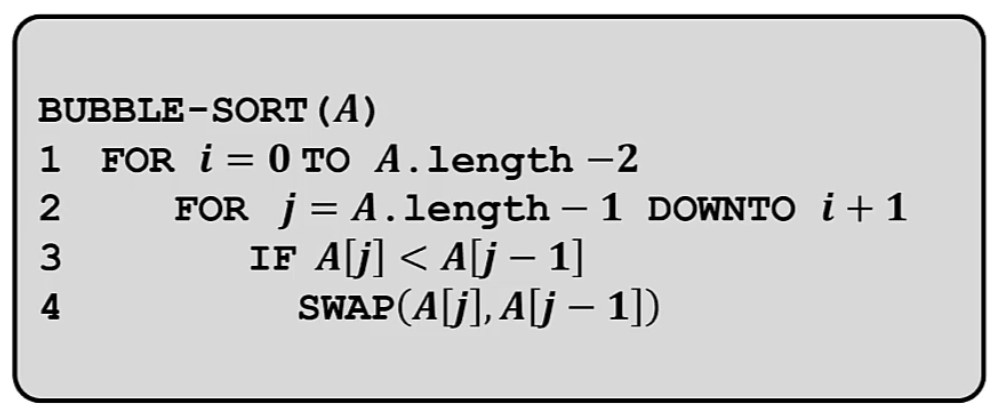
\includegraphics[scale=0.4]{BubbleSort_Code.jpg}
				\end{center}
		\end{minipage}
				
		\subsubsection{Analyse}
			Anzahl der Vergleiche
			\begin{itemize}
				\item es werden stets alle Elemente er Teilfolge verglichen
				\item unabhängig von der Sortierung
			\end{itemize}
			Anzahl der Vertauschungen
			\begin{itemize}
				\item Best case: 0 Vertauschungen
				\item Worst case: $\frac{n^2 - n}{2}$ Vertauschungen
			\end{itemize}
			Komplexität
			\begin{itemize}
				\item Best case: $\Theta (n)$
				\item Average case: $\Theta (n^2)$
				\item Worst case: $\Theta (n^2)$
			\end{itemize}
			\vspace{1.5cm}
		
		
	\subsection{SelectionSort}
		\subsubsection{Grundidee}
			$\rhd$ Sortieren durch direktes Auswählen
				
			\begin{itemize}
				\item MinSort: "wähle kleinstes Element in Array und tausche es nach vorne
				\item MaxSort: "wähle grö\ss etes Element in Array und tausche es nach hinten
			\end{itemize}
				
		\subsubsection{Code}
			\begin{center}
				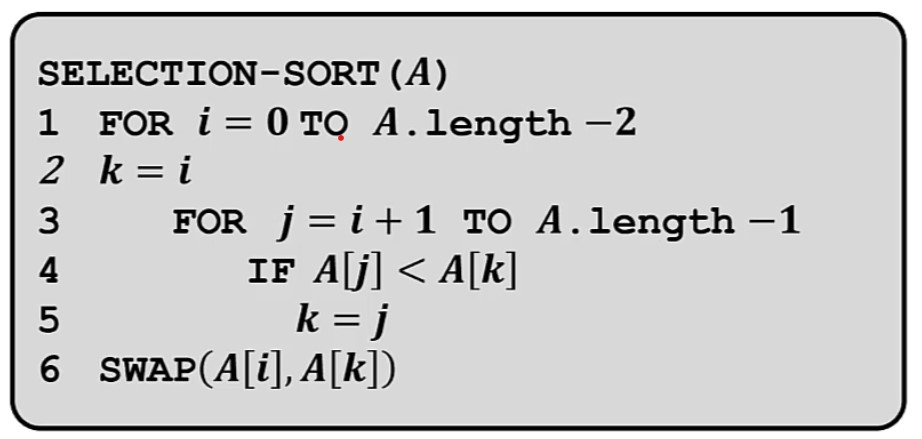
\includegraphics[scale=0.5]{SelectionSort_Code.jpg}
			\end{center}
			\vspace{1.5cm}
		
		
	\subsection{MergeSort}
		\label{MergeSort}
		
		\subsubsection{Grundidee}
			$\rhd$ Baut auf dem Devide-and-Conquer Prinziep auf
			\begin{itemize}
				\item \textbf{Divide:} Teile die Folge mit $n$ Elementen in zwei Teilfolgen von je $\frac{n}{2}$ Elementen auf
				\item \textbf{Conquer:} Sortiere die zwei Teilfolgen rekursiv mithilfe von MergeSort
				\item Vereinige die zwei sortierten Teilfolgen, um die sortierte Lösung zu erzeugen
			\end{itemize}
				
				
		\subsubsection{Code}
			\begin{center}
				Prinziep des MergeSorts \\
				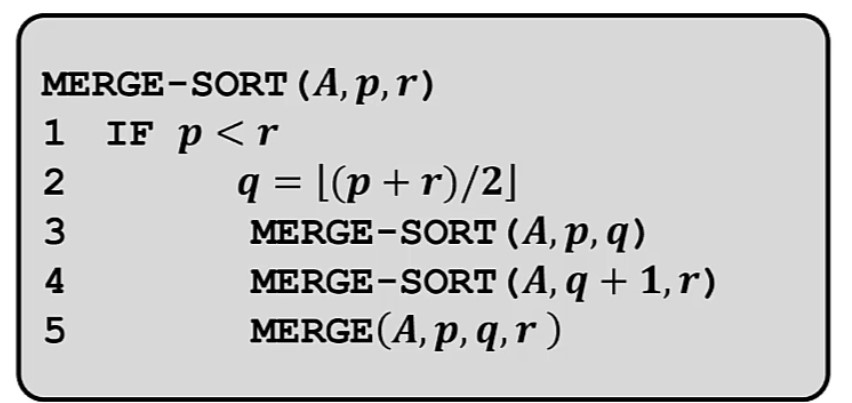
\includegraphics[scale=0.53]{MergeSort_Code.jpg}
			\end{center}
			\mbox{} \\
			Beim Halbieren wird immer abgerundet, so kann jede Teilfolge sortiert werden. \\ \\
				
			\begin{center}
				Prinziep des gesamtes Codes \\
				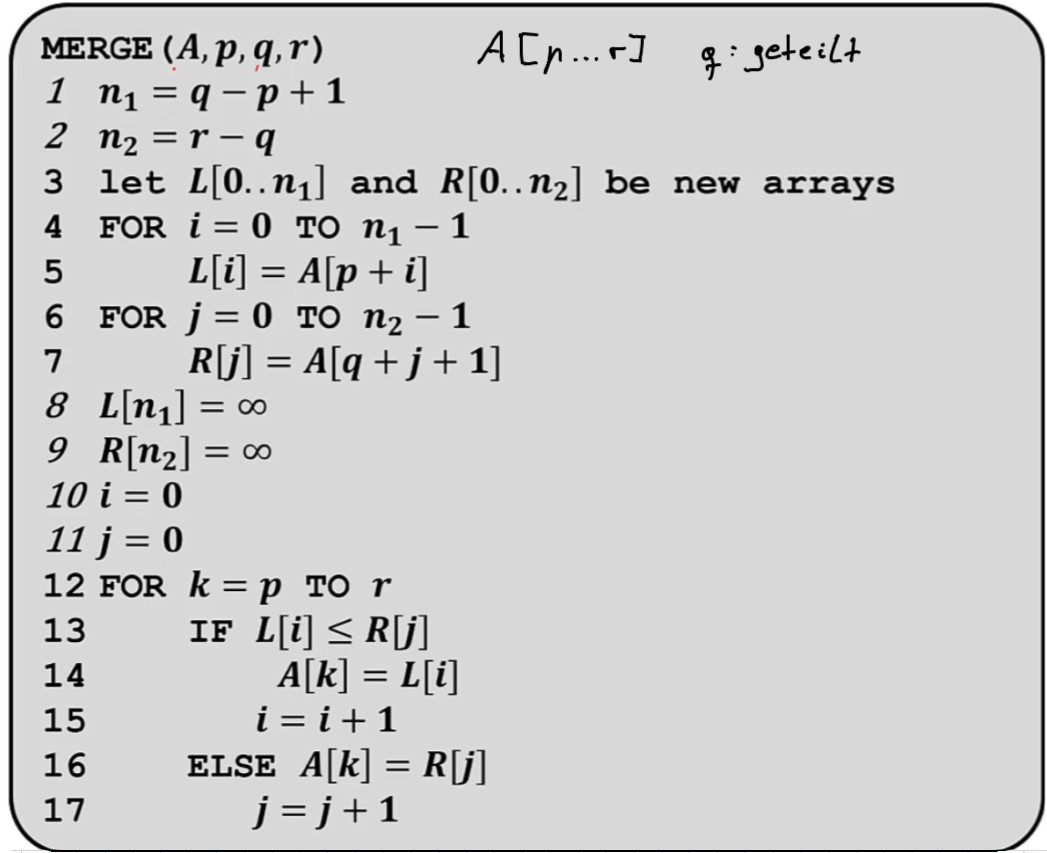
\includegraphics[scale=0.5]{MergeSort_Komplett_Code.jpg}
			\end{center}
			\mbox{} \\ \\
				
				
		\subsubsection{Analyse}
			\textbf{Ziel:} Bestimme Rekursionsgleichung für Laufzeit $T(n)$ von $n$ Zahlen im schlechtesten Fall
			\begin{itemize}
				\item \textbf{Divide:} Es wird einfach die Mitte des Feldes berechnet. Dies benötigt konstante Zeit, also $\Theta(1)$
				\item \textbf{Conquer:} Wir lösen zwei Teilprobleme der Grö\ss e $\frac{n}{2}$ rekursiv. Dies trägt mit $2T(\frac{n}{2})$ uir Laufzeit bei
				\item \textbf{Combine:} Die Prozedur \texttt{MERGE} auf einem Teilfeld der Länge $n$ lineare Zeit, also $\Theta(n)$
			\end{itemize}
				
			\begin{center}
				\[
					T(n) = \left\{\begin{array}{lr}
						c & \text{falls } n = 1 \\
						2T(\frac{n}{2}) + cn & \text{falls } n > 1 
					\end{array}\right\}
					\] \vspace{0.35cm}
						
					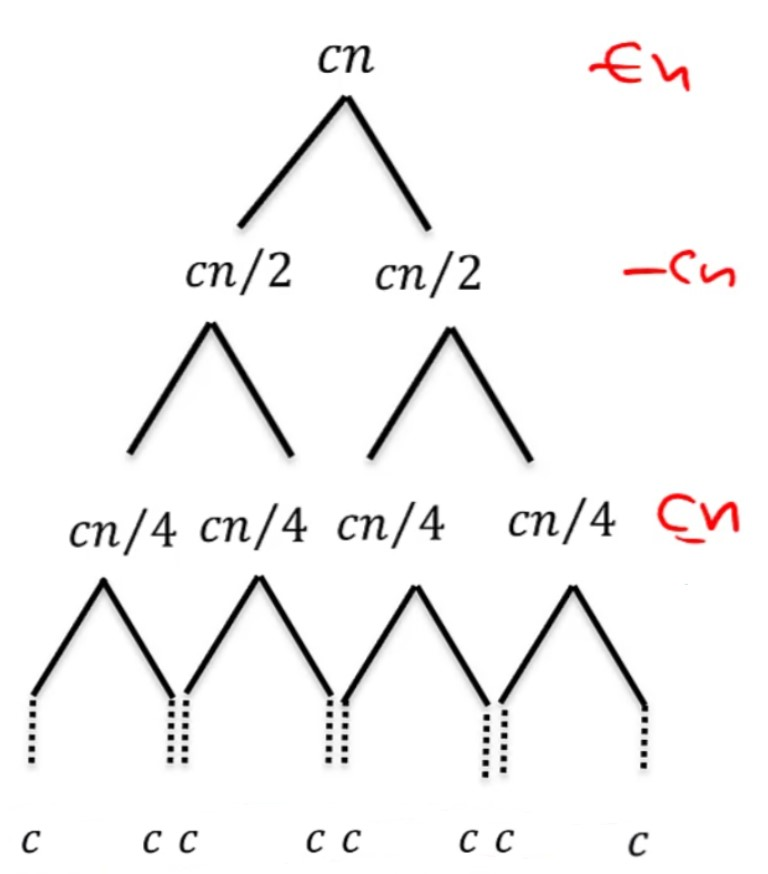
\includegraphics[scale=0.35]{MergeSort_BinaryTree.jpg}
				\end{center}
					
				Daraus ergibt sich eine Komplexität von $\Theta(n \log n)$ \\
				
					
					
		\subsubsection{Beweis der Korrektheit}
			\textbf{Schleifeninvariante:} Zu Beginn jeder Iteration der for-Schleife (Zeile 12-17) enthält 
			das Teilfeld $A[p...k-1]$ die $k-p$ kleinsten Elemente aus $L[0...n_1]$ und $R[0...n_2]$ 
			in sortierter Reihenfolge. Weiter sind $L[i]$ und $R[j]$ die kleinsten Elemente ihrer 
			Arrays, die noch nicht zurück kopiert wurden. \\ \\
			\textbf{Initialisierung:} Vor der ersten Iteration gilt $k = p$. \\ Daher ist $A[p...k-1]$
			leer und enthält $0$ kleinste Elemente von $L$ und $R$. Wegen $i = j = 0$ sind $L[i]$ und
			$R[j]$ die kleinsten Elemente ihrer Arrays, die noch nicht zurück kopiert wurde. \\ \\
			\textbf{Fortsetzung:} Müssen zeigen, dass Schleifeninvariante erhalten bleibt. Dafür nehmen wir an,
			dass $L[i] \leq R[j]$. Dann ist $L[i]$ kleinstes Element, welches noch nicht zurück kopiret wurde.
			Da Array $A[p...k-1]$ die $k - p$ kleinsten Elemente enthält, wird der Array $A[p...k]$ die 
			$k - p + 1$ kleinsten Elemente enthalten nachdem der Wert nach der Durchführung von Zeile 14 
			kopiert wurde. Nach Erhöung der Variablen $k$ und $i$ stellt die Schleifeninvariante für die 
			nächste Iteration wieder her. \\ Wenn $L[i] > R[j]$ dann analoges Argument mit Zeilen 16-17. \\ \\
			\textbf{Terminierung:} Beim Abbruch gilt $k = r + 1$. Durch die Schleifeninvariante enthält 
			$A[p...r]$ die kleinsten Elemente von $L[0...n_1]$ und $R[0...n_2]$ in sortierter Reihenfolge.
			Alle Elemente au\ss er der Sentinels wurden korrekt zurück kopiert.
			\vspace{1.5cm}
		
		
	\subsection{QuickSort}
		\begin{minipage}[t]{0.5\textwidth}
			\subsubsection{Grundidee}
				\begin{itemize}
					\item Wähle ein Pivotelement $x$ des Arrays
					\item Zerlege den Array in zwei Teilarrays
					\begin{itemize}
						\item Erster Teilarray: Enthält alle Elemente $y \leq x$
						\item Zweiter Teilarray: Enthält alle Elemente $y > x$ 
					\end{itemize}
					\item Sortiere rekursiv auf den Teillisten mit Quicksort
					\item Einelementige Listen sin schon sortiert
				\end{itemize}
			\end{minipage}
			\begin{minipage}[t]{0.45\textwidth}
				\subsubsection{Eigenschaften}
					\begin{itemize}
						\item Instabiler Sortieralgorithmus
						\item Basiert auf Divide and Conquer
					\end{itemize}
			\end{minipage}
		
		\subsubsection{Divide-and-Conquer}
			\begin{itemize}
				\item \textbf{Divide:} Zerlege das Array $A[p...r]$ in zwei Teilarrays $A[p...q-1]$ 
					und $A[q+1...r]$, sodass jedes Element aus $A[p...q-1]$ kleiner oder gleich $A[q]$
					ist, welches wiederum kleiner oder gleich jedem Element von $A[q+1...r]$ ist. 
					Berechnen den Index $q$ als Teil vom Partition Algorithmus.
				\item \textbf{Conquer:} Sortieren beider Teilarrays $A[p...q-1]$ und $A[q+1...r]$ durch
					rekursiven Aufruf von Quicksort
				\item \textbf{Combine:} Da die Teilarrays bereits sortiert sind, ist keine weitere Arbeit
					nötig um diese zu vereinigen. $A[p...r]$ ist nun sortiert. 
			\end{itemize}
					
		
		\subsubsection{Code}
			\begin{minipage}[t]{0.5\textwidth}
				\begin{center}
					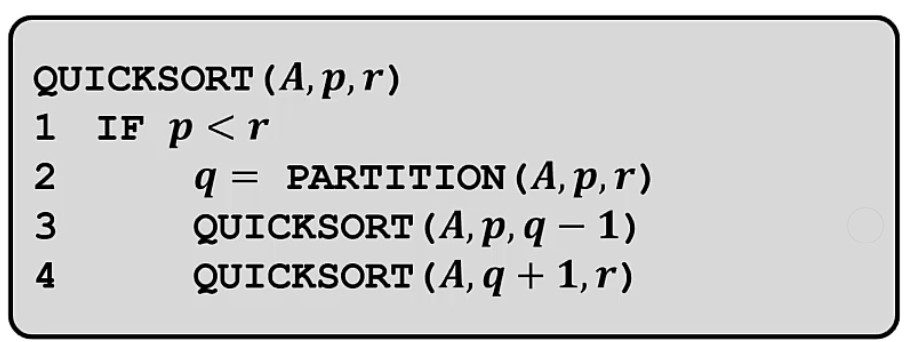
\includegraphics[scale=0.5]{QuickSort_Code_Partition.jpg} \\ \vspace{0.5cm}
					Im Folgenden gucken wir uns den Algorithmus genauer an $\Rightarrow$ \\ \vspace{0.5cm}
				\end{center}
			\end{minipage}
			\begin{minipage}[t]{0.45\textwidth}
				\begin{center}
					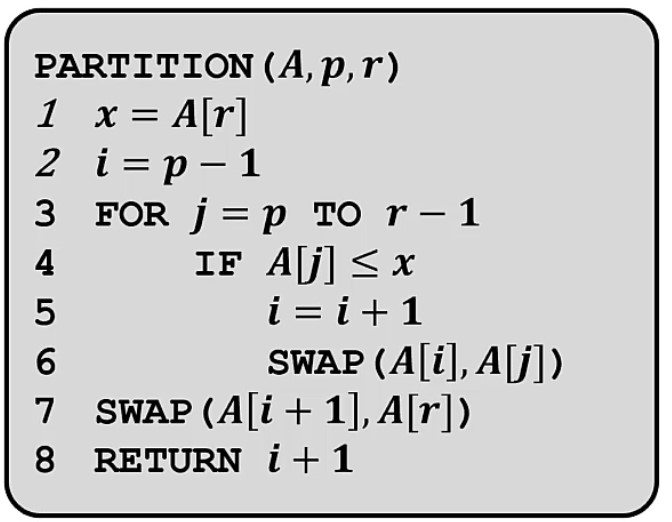
\includegraphics[scale=0.4]{QuickSort_Code.jpg} \\ \vspace{0.5cm}
					Zeile 1: Pivotelement wählen \\
					Zeile 2: Index $i$ setzen \\
					Zeile 3-6: Teilarrays mit Element füllen \\
					Zeile 7: Pivotelement tauschen \\
					Zeile 8: Neuer Index des Pivotelements \\ \vspace{0.9cm}
				\end{center}
			\end{minipage} \\
		
			\begin{minipage}{0.5\textwidth}
				\begin{center}
					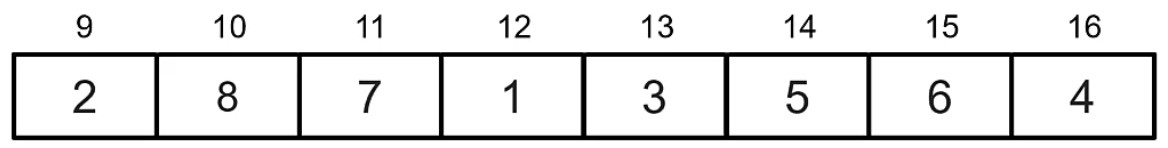
\includegraphics[scale=0.35]{QuickSort_Code_PartitionSample_01.jpg} \\
					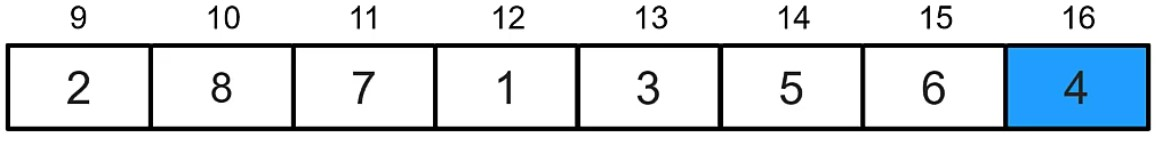
\includegraphics[scale=0.35]{QuickSort_Code_PartitionSample_02.jpg} \\
				\end{center}
			\end{minipage}
			\begin{minipage}{0.05\textwidth}
				\begin{center}
					$\Rightarrow$
				\end{center}
			\end{minipage}
			\begin{minipage}{0.45\textwidth}
				\begin{center}
					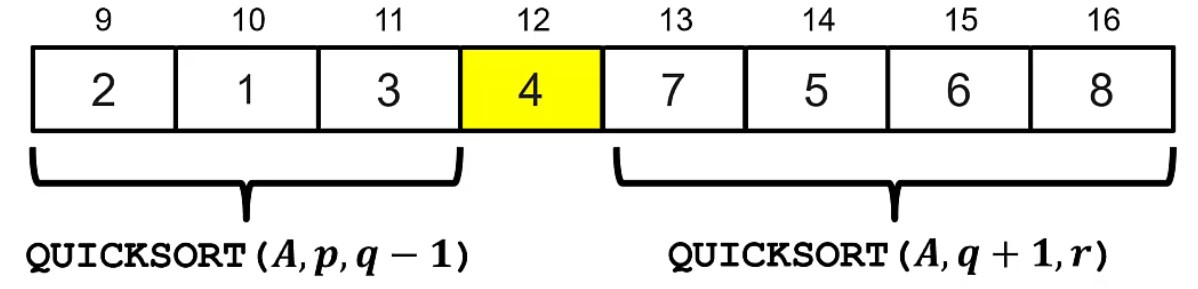
\includegraphics[scale=0.35]{QuickSort_Code_PartitionSample_00.jpg} \\
				\end{center}
			\end{minipage}
		
		
		\subsubsection{Korrektheit von Quicksort}
			\begin{itemize}
				\item \textbf{Schleifeninvariante:} Zu Beginn jeder Iteration der for-Schleife (Zeile3-6)
					gilt für den Arrayindex $k$ folgendes:
				\begin{itemize}
					\item Ist $p \leq k \leq i$, so gilt $A[k] \leq x$.
					\item Ist $i + 1 \leq k \leq j - 1$, so gilt $A[k] > x$.
					\item Ist $k = r $, so gilt $A[k] = x$.
				\end{itemize}
				\item \textbf{Initialisierung:} Vor der ersten Iteration gilt $i = p-1$ und $j = p$.
					Da es keine Werte zwischen $p$ und $j$ gibt und es auch keine Werte zwischen $i+1$ 
					und $j-1$ gibt, sind die ersten beiden Eigenschaften trivial erfüllt. \\
					Die Zuweisung in Zeile 1 sorgt für die Erfüllung der dritten Eigenschaft.
				\item \textbf{Fortsetzung:} Zwei mögliche Fälle durch Zeile 4. \\
					Wenn $A[j] > x$, dann inkrementiert die Schleife ur den Index $j$ . Dann gilt Bedingung 2
					für $A[j-1]$ und alle anderen Einträge bleiben unverändert. \\
					Wenn $A[j] \leq x$, dann wird index $i$ inkrementiert und die Einträge $A[i]$ und $A[j]$
					getauscht und schlie\ss lich der Index $j$ erhöht. Wegen des Vertauschens gilt 
					$A[i] \leq x$ und Bedingung 1 ist erfült. Analog gilt $A[j-1] > x$, da das Element welches
					mit $Aj-1]$ vertauscht wurde wegen der Invariante gerade grö\ss er als $x$ ist.
				\item \textbf{Terminierung:} Bei der Terminierung gilt, dass $j=r$. Daher gilt, dass
					jeder Eintrag des Arrays zu einer der drei durch die Invariante beschriebenen Menge gehört.
				\end{itemize}
				\vspace{1.5cm}


\newpage
\section{Datenstrukturen}
	\subsection{Datenstrukturen: Theorie}
		\subsubsection{Definiton}
			\begin{center}
				Eine Datenstruktur ist eine Methode, Daten abzuspeichern und zu \\
				organisieren sowie den Zugriff auf die Daten un die Modifikation der Daten zu erleichtern
			\end{center}
			

		\subsubsection{Besipiele}
			\begin{center}
				\begin{tabular}{ p{4cm} | p{4cm} | p{4cm} }
					\makecell[c] {\textbf{Grundlegende} \\ \textbf{Datenstrukturen}} &
					\makecell[c] {\textbf{Fortgeschrittene} \\ \textbf{Datenstrukturen}} &
					\makecell[c] {\textbf{Randomisierte} \\ \textbf{Datenstrukturen}} \\

					\makecell[c] {Stacks} &
					\makecell[c] {Rot-Schwarz-Bäume} &
					\makecell[c] {Skip Lists} \\
			
					\makecell[c] {Verkettete Listen} &
					\makecell[c] {AVL-Bäume} &
					\makecell[c] {Hash Tables} \\

					\makecell[c] {Queues} &
					\makecell[c] {Splay-Bäume} &
					\makecell[c] {Bloom-Filter} \\

					\makecell[c] {Bäume} &
					\makecell[c] {Heaps} &
					\makecell[c] {} \\

					\makecell[c] {Binäre Suchbäume} &
					\makecell[c] {B-Bäume} &
					\makecell[c] {} \\
				\end{tabular}
			\end{center}
			\vspace{1cm}

		\subsubsection{Begriffsunterscheidung}
			Abstrakter Datentyp ("was") \\
			Beschreibt Stack mit Operationen \\
			Datenstrukturen ("wie") \\
			Beschreibt die Stack-Operationen als Array oder Verkettete Liste

	\vspace{1.5cm}

	\subsection{Stacks}
		\subsubsection{Operationen:}
			\begin{itemize}
				\item new(S)		- erzeugt neuen (leeren) Stack
				\item isEmpty(S)	- gibt an, ob Stack S leer ist
				\item pop(S)		- gibt oberstes Element vom Stack S zurück und löscht es, falls vorhanden
				\item push(S,k)		- schreibt k als neues oberstes Element auf S
				\item $\longrightarrow$ LIFO - last in, first out
			\end{itemize}
			\begin{center}
				Intuitive erwartete Bedingugen sind erfüllt, auch ohne algebraische Spezifikiation
			\end{center}

		\subsubsection{Darstellung als Array} 
			\begin{center}
				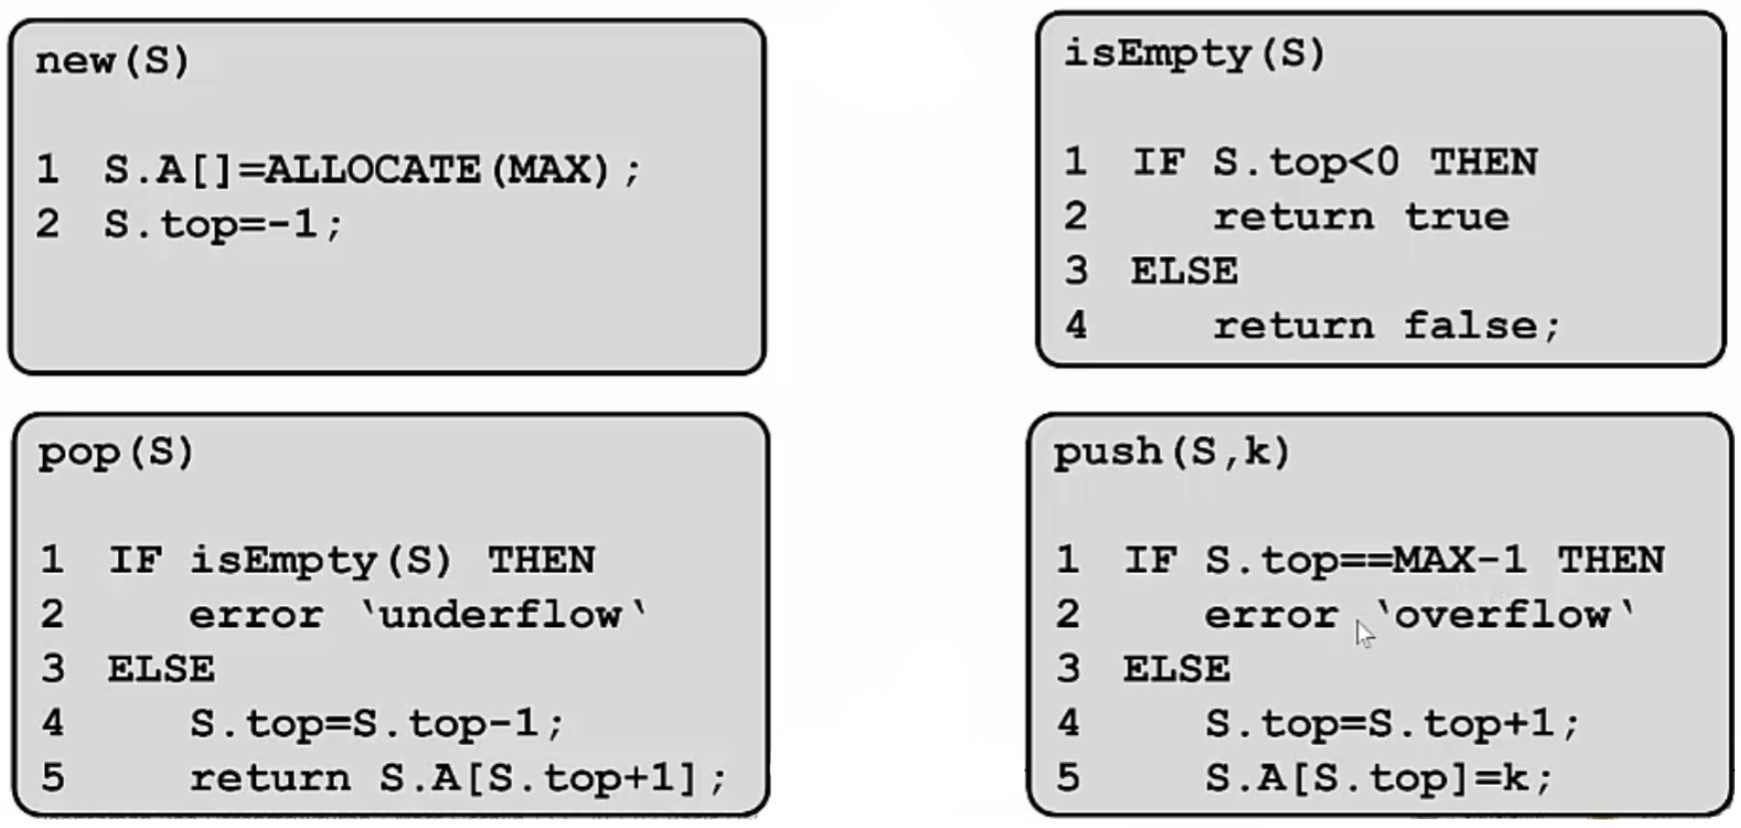
\includegraphics[scale=0.4]{Stack_Operationen_Code.jpg}
			\end{center}

			\paragraph{} Bei der Darstellung als Array kann die maximale Grö\ss e erreicht werden. Danach wird beim 
			Hin zufügen das ganze Array in ein größeres kopiert. Da dies in $\Theta (n^2)$ liegt wird ein
			Faktor festgelegt. So wird beispielweise bei erreichen der maximalen Grö\ss e die Grö\ss e
			verdoppelt, haben wir weniger als 1/Faktor*Faktor, also weniger als ein Viertel der Elemente belegt
			so halbieren wir unser Array.


			\vspace{1.5cm}


	\subsection{Verkettete Listen}
		\begin{minipage}[t]{0.5\textwidth}
			\subsubsection{Darstellung:}
				\begin{center}
					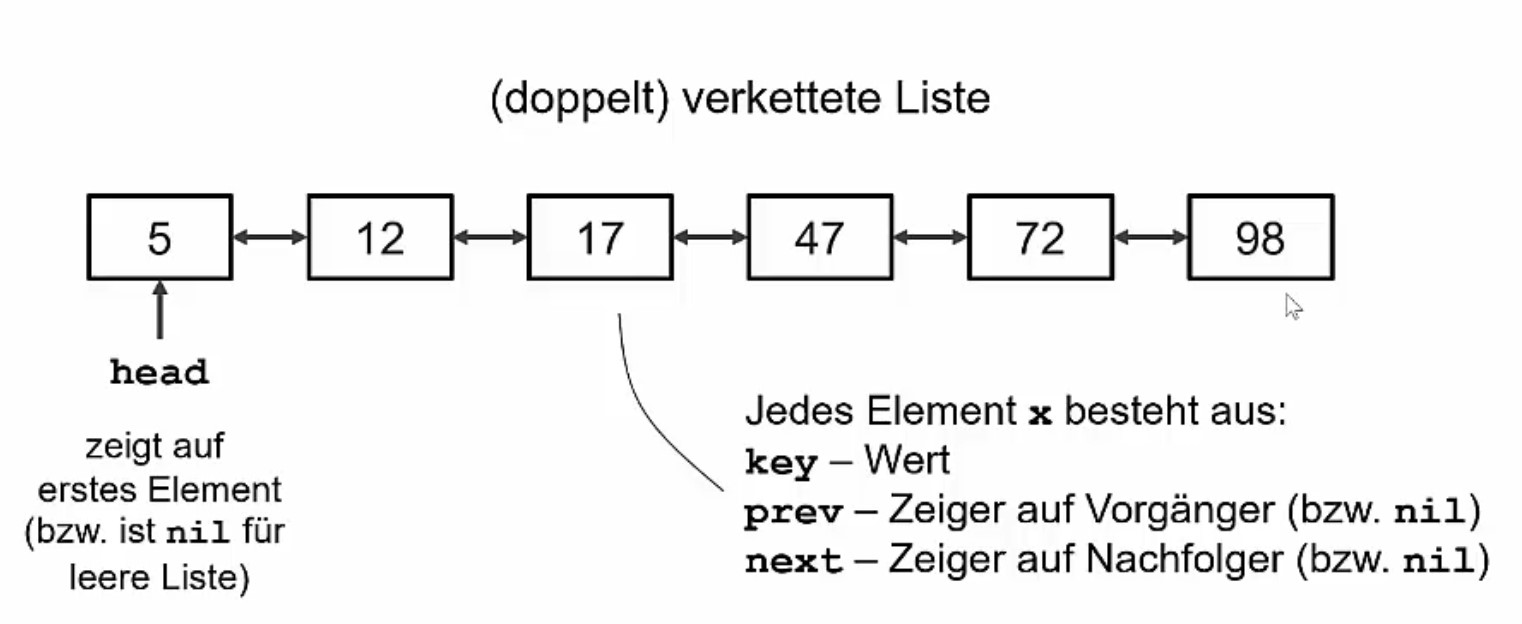
\includegraphics[scale=0.35]{Doppelt_Verkettete_Listen_Bsp.jpg}
				\end{center}
		\end{minipage}
		\begin{minipage}[t]{0.45\textwidth}
			\begin{center}
				\subsubsection{Operationen und Laufzeit:}
				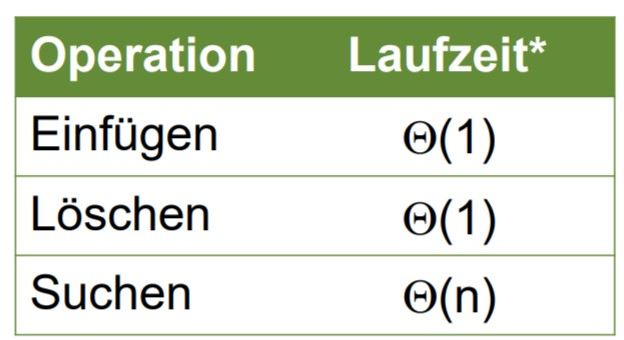
\includegraphics[scale=0.4]{LinkedListLaufzeit.jpg}
			\end{center}
		\end{minipage}

		\vspace{1.5cm}

	

	\subsection{Queues}
		\subsubsection{Operationen:}
			\begin{itemize}
				\item new(Q) - erzeugt neue (leere) Queue
				\item isEmpty(Q) - gibt an, ob Queue leer ist
				\item dequeue(Q) - gibt vorderstes Element der Queue zurück und löscht es
				\item enqueue(Q,k) - schreibt k als neuees hinterstes Element auf Q
				\item $\longrightarrow$ FIFO - first in, first out
			\end{itemize}

		\subsubsection{Darstellung als Array}
			Bei der Darstellung als Array stö\ss t man nun auf Probleme. Es werden nun zwei Zeiger, 
			und nicht mehr wie bei Stacks nur einer, benötigt. Da die Schlange aber nun durch das 
			Array durchwandert bleibt sehr viel Arrrayplatz ungenutzt, bzw. man bräuchte ein unendlich
			gro\ss es Array. Daher gibt es zwei Darstellungsmöglichkeiten:
			\begin{center}
				Als Array: \hspace{5cm} Als zyklisches Array:\\
				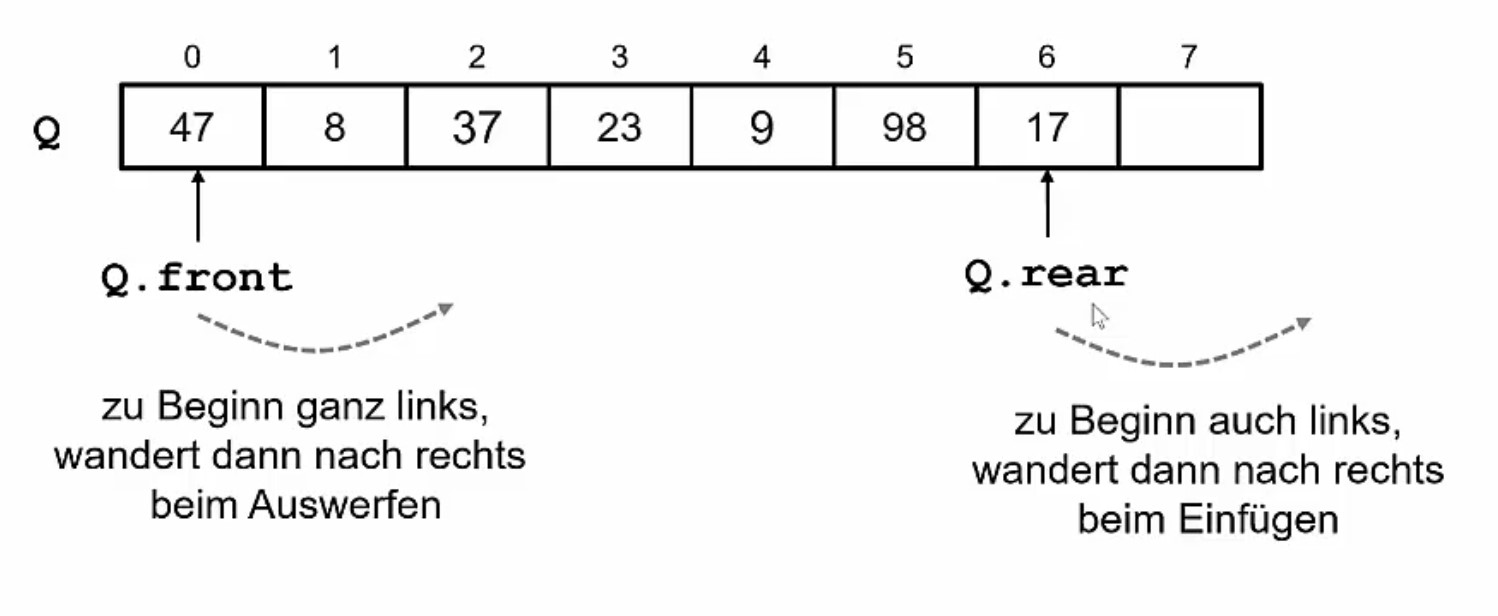
\includegraphics[scale=0.3]{Queues_Array.jpg}
				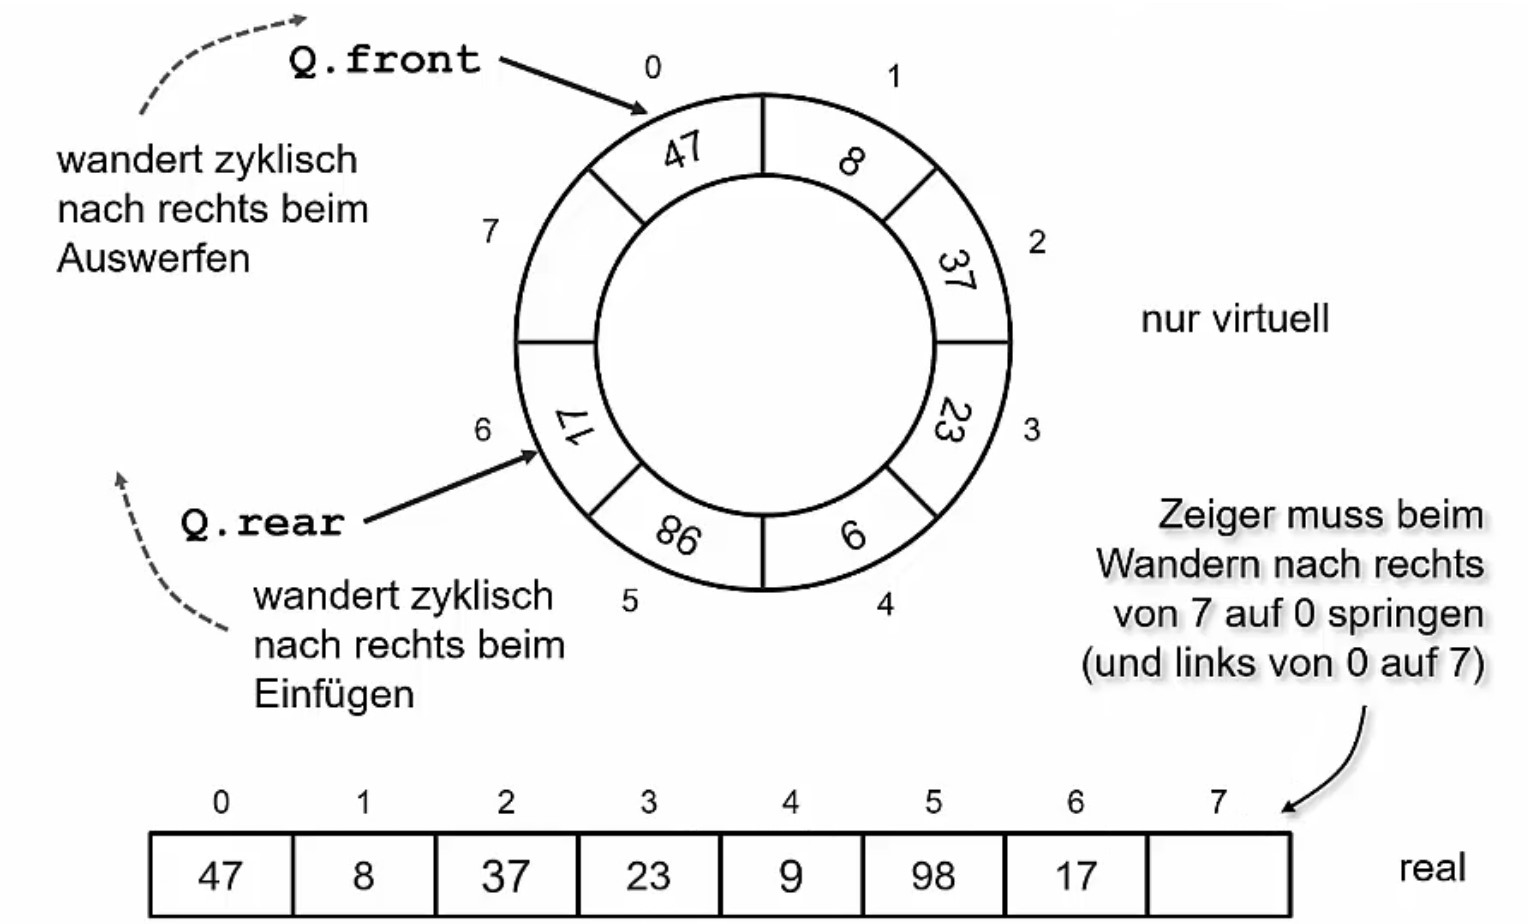
\includegraphics[scale=0.3]{Queues_Array_Zyklisch.jpg}
			\end{center}

			\vspace{1.5cm}

	
	\subsection{Binärbäume - Bäume}
		\begin{minipage}[t]{0.5\textwidth}
			\subsubsection{Eigenschaften und Begrifflichkeiten}
				\begin{itemize}
					\item Jeder Knoten ist eindeutig zu erreichen $\Rightarrow$ azyklischer Graph
					\item Root, Leaf, Child, Descendent, Parent, Ancestor, Sinbling $\Rightarrow$
					\item Halbblatt: Ein Knoten der genau ein Kind hat
				\end{itemize}

		
			\hspace{3cm}	
			\subsubsection{Charackteristik}
				\begin{center}
					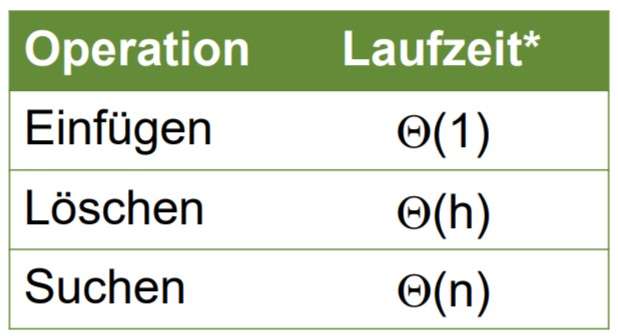
\includegraphics[scale=0.4]{BBCharackterisitk.jpg}
				\end{center}
		\end{minipage}
		\hspace{0.5cm}
		\begin{minipage}[t]{0.45\textwidth}
			\begin{center}
			\subsubsection{Darstellung als Ungerichteter Graph}
				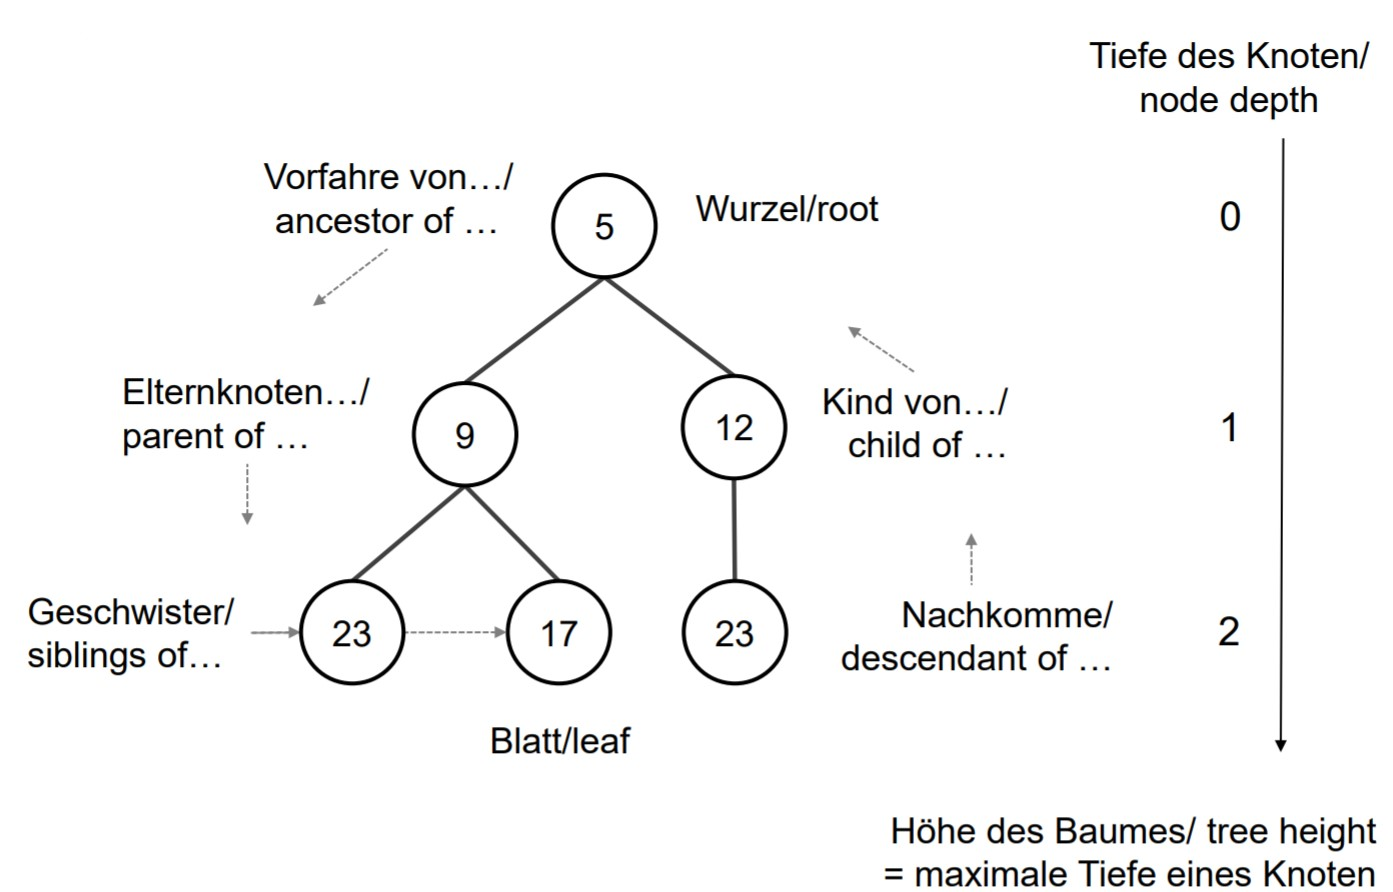
\includegraphics[scale=0.35]{BinaerBaeumeGraph.jpg}
			\end{center}

			\subsubsection{Höhe/Tiefe}
				\begin{itemize}
					\item Höhe des Leeren Baums per Konvention = -1
					\item Höhe (nicht leerer) Baum = max {Höhe aller Teilbäume der Wurzel} + 1
				\end{itemize}
		\end{minipage} \\

		\vspace{1cm}

		\begin{minipage}[t]{0.5\textwidth}
			\subsubsection{Inorder-Traversieren von Binärbäumen}
				\paragraph{} Das Inorder-Traversieren ist eine Möglichkeit durch alle Knoten eines Binärbaums 
				zu Iterieren. Die Laufzeit beträgt O(n). Dabei ist diese Vorgehensweise nicht eindeutig, das hei\ss t
				mehrere Bäume können die gleiche Inorder-Traversierung haben. \\
				Im allgemeinen werden die Knoten dabei in aufsteigender Reihenfolge ausgegeben. \\ \\ 

				\textbf{Bemerkung:} Genauso gibt es noch Pre- und Postorder
		\end{minipage}
		\begin{minipage}[t]{0.45\textwidth}
			\begin{center}
			\subsubsection{Inorder-Traversierung mit Beispiel}
				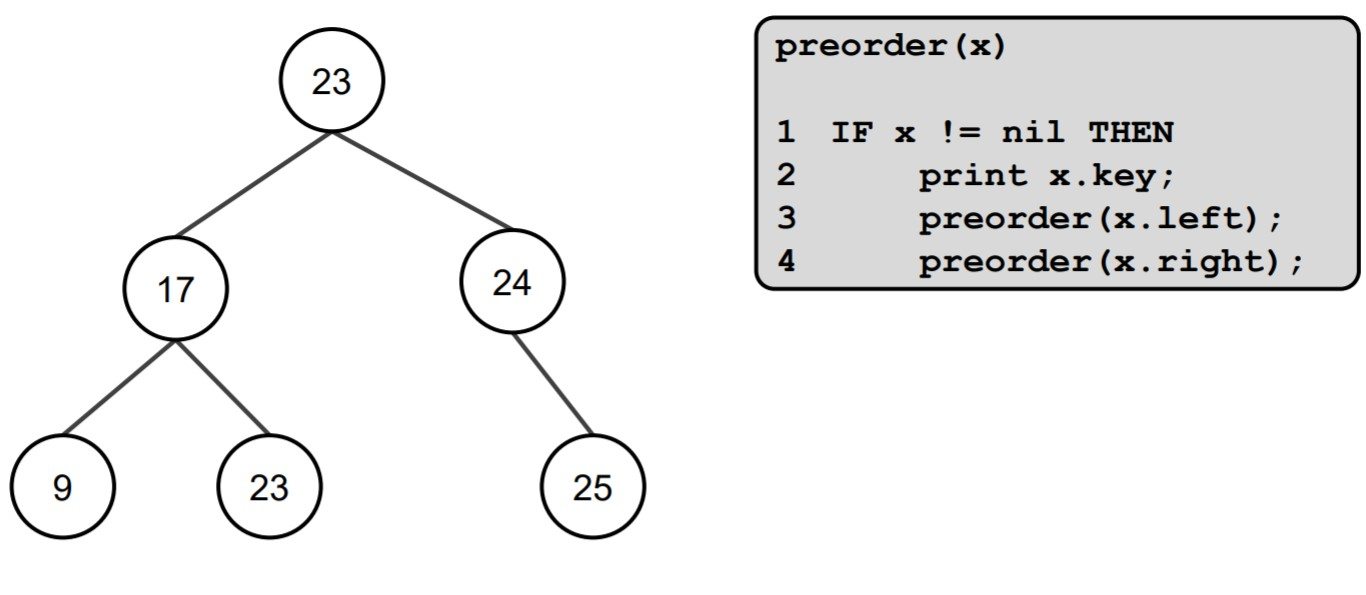
\includegraphics[scale=0.4]{BBInorder.jpg}
				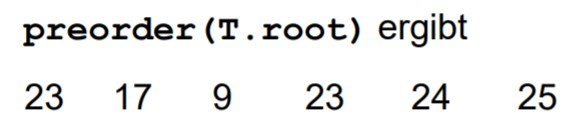
\includegraphics[scale=0.4]{BBInorderErgebniss.jpg}
			\end{center}
		\end{minipage}

		\begin{center}
			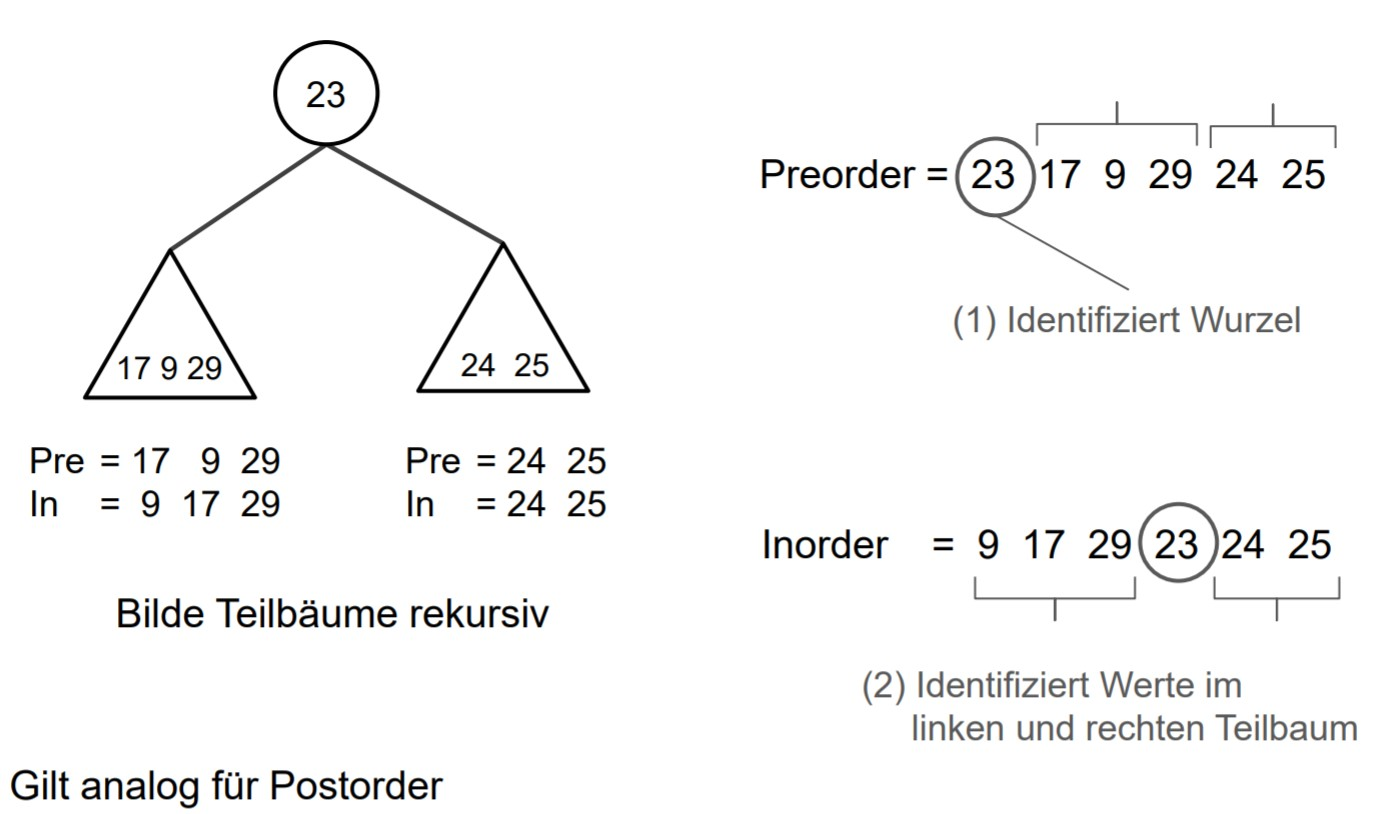
\includegraphics[scale=0.35]{BBTraversieren.jpg}
			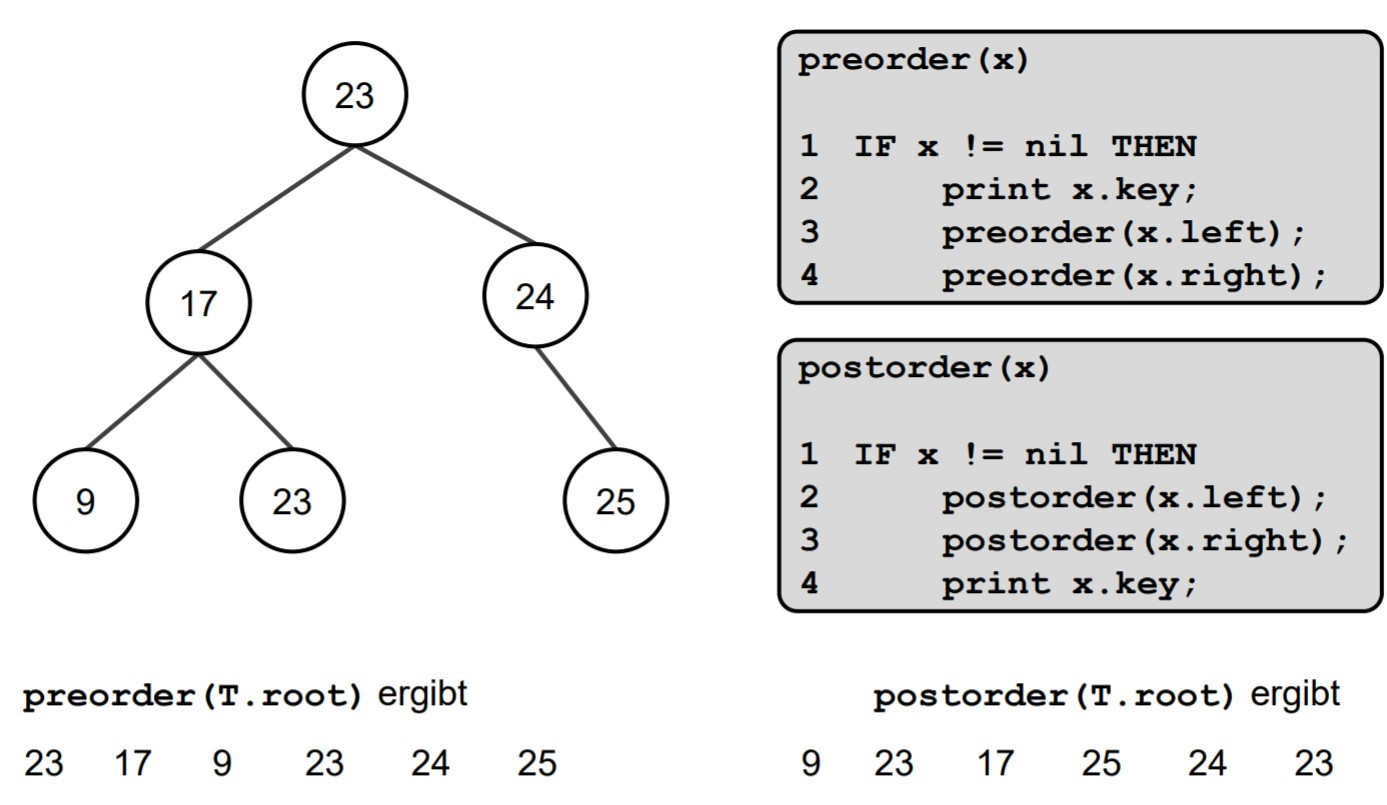
\includegraphics[scale=0.35]{BBPrePostorder.jpg}
		\end{center}

	
	\newpage
	\subsection{Binäre-Suchbäume}
		\subsubsection{Eigenschaften}
			\begin{itemize}
				\item Ein Binärersuchbaum basiert auf dem Prinziep eines Binärbaums \\
					Heirbei gilt jedoch für jeden Knoten, dass der Wert seines rechten Kindes 
					mindestens so groß sein muss wie der Werte des Knoten. Umgekehrt gilt dies auch 
					für das Linke kind.
				\item Sei x Knoten im linken Teilbaum von z $\Rightarrow$ \texttt{x.key $\leq$ z.key}
				\item Sei y Knoten im linken Teilbaum von z $\Rightarrow$ \texttt{y.key $\geq$ z.key}
			\end{itemize}


		\begin{minipage}[t]{0.45\textwidth}
			\subsubsection{Suchen}
				\begin{itemize}
					\item Durch die teilsortierung, also die Bedingung eines Binärensuchbaums, 
						kann der Suchbereich auf Teilbäume eingegrenzt werden.
				\end{itemize}
				\begin{center}
					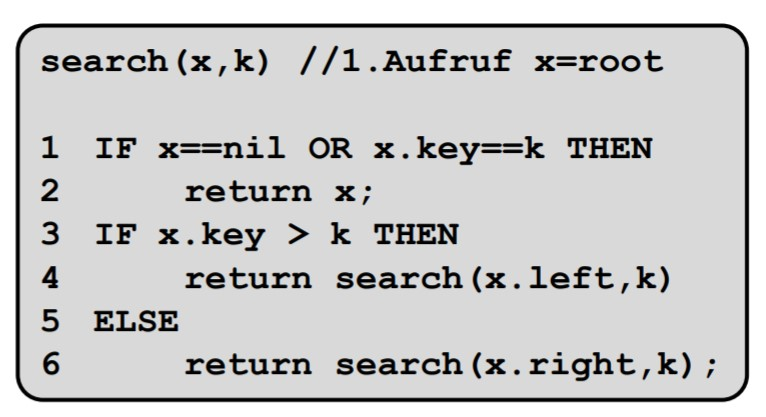
\includegraphics[scale=0.3]{BSBSearch.jpg}
				\end{center}
		\end{minipage}
		\begin{minipage}[t]{0.1\textwidth}
			\hspace{0.5cm}
		\end{minipage}
		\begin{minipage}[t]{0.45\textwidth}
			\subsubsection{Einfügen}
				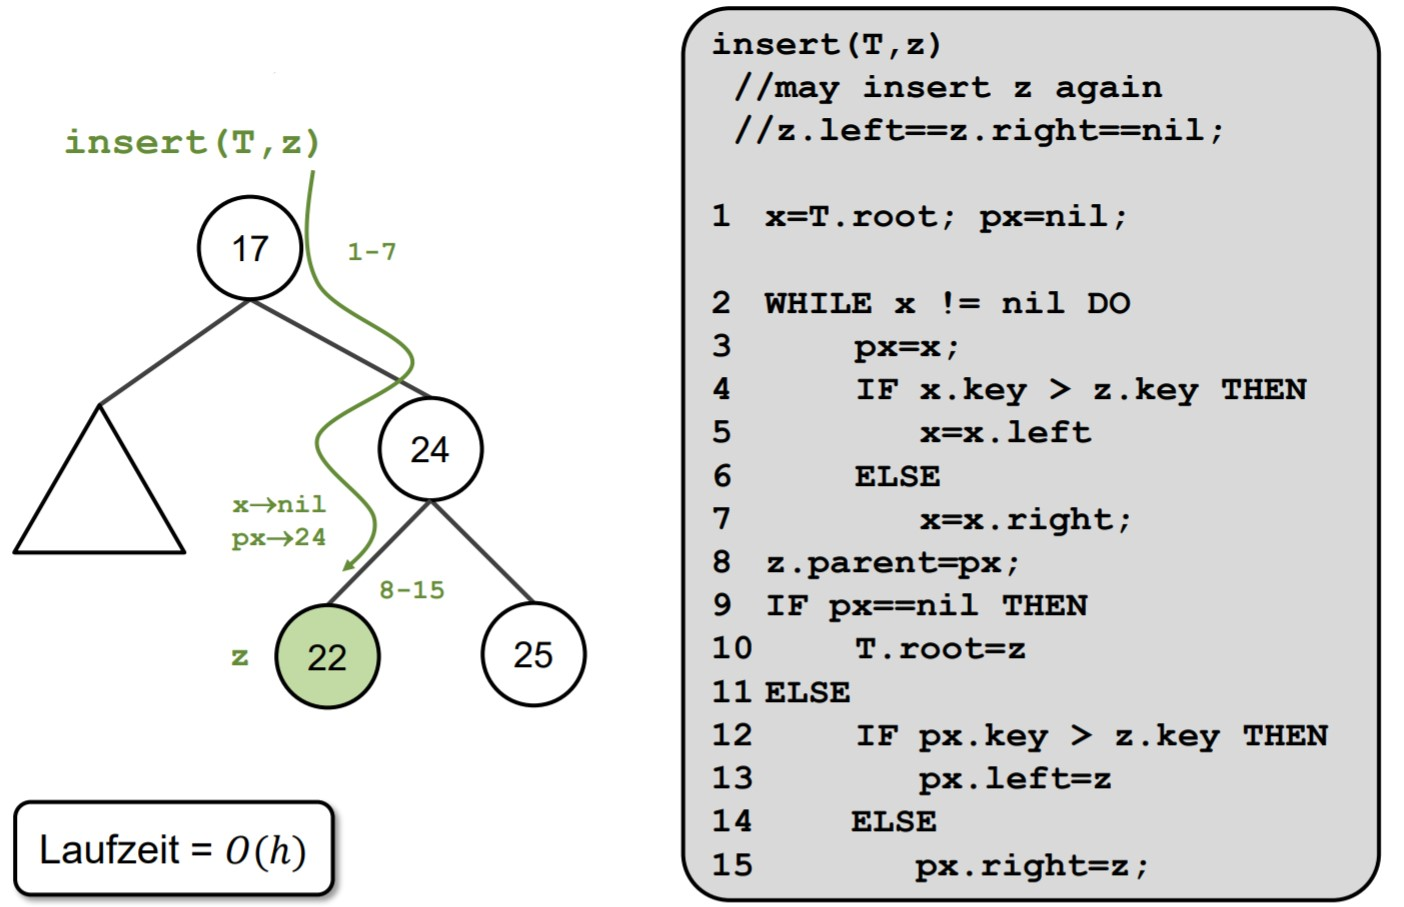
\includegraphics[scale=0.3]{BSBInsert.jpg}
		\end{minipage}

		\vspace{1.5cm}

		\begin{minipage}[t]{0.35\textwidth}
			\subsubsection{Löschen: Transplant}
				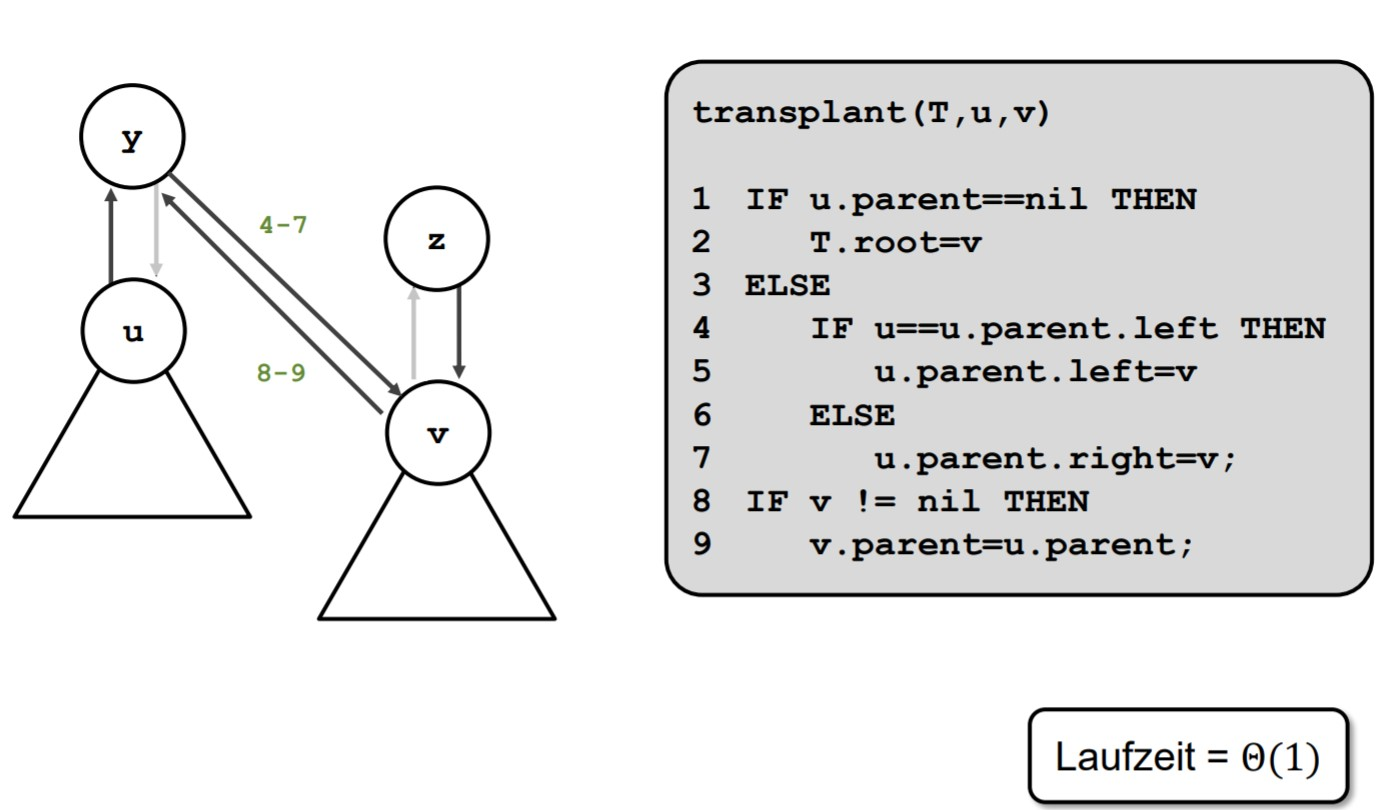
\includegraphics[scale=0.3]{BSBTransplant.jpg}

			\vspace{1cm}
			\subsubsection{Charackteristik}
				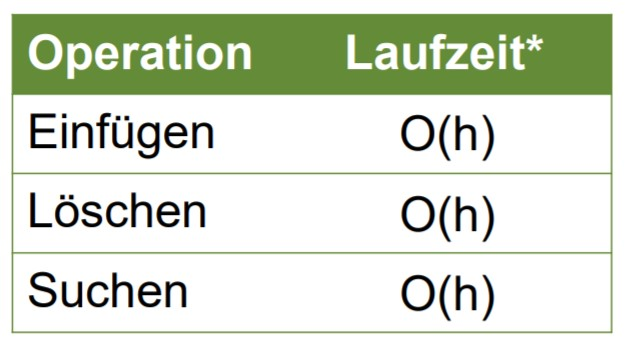
\includegraphics[scale=0.4]{BSBCharackterisitk.jpg}
		\end{minipage}
		\begin{minipage}[t]{0.1\textwidth}
			\hspace{0.5cm}
		\end{minipage}
		\begin{minipage}[t]{0.55\textwidth}
			\subsubsection{Löschen}
				\begin{center}
					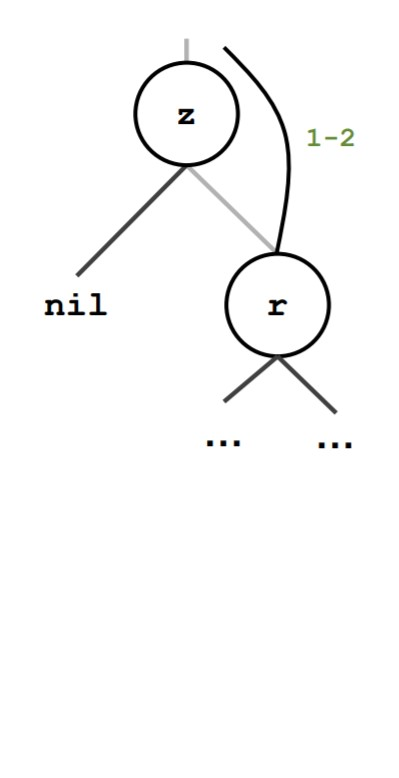
\includegraphics[scale=0.3]{BSBDelete01.jpg}
					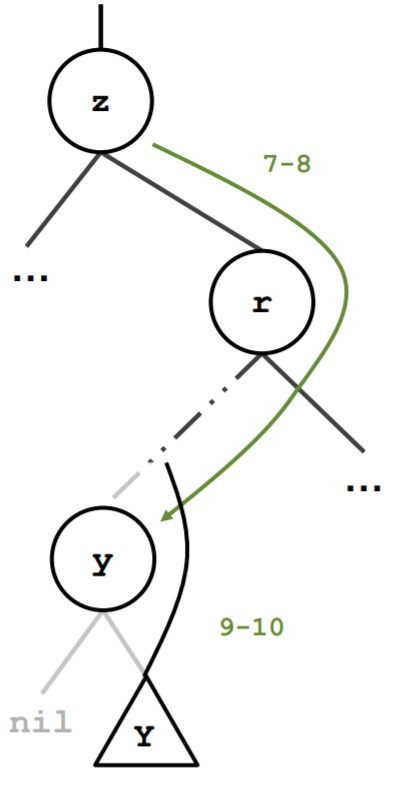
\includegraphics[scale=0.3]{BSBDelete02.jpg}
					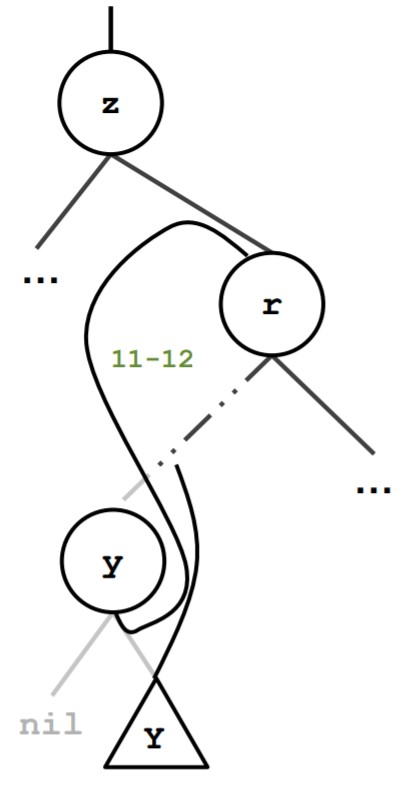
\includegraphics[scale=0.3]{BSBDelete03.jpg}
					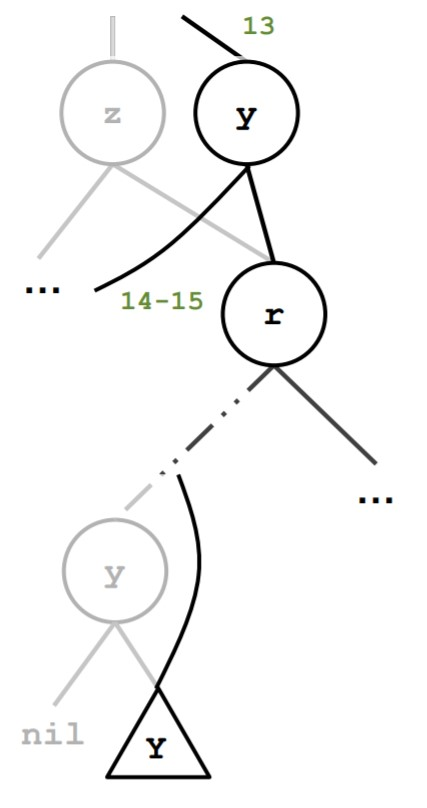
\includegraphics[scale=0.3]{BSBDelete04.jpg}
					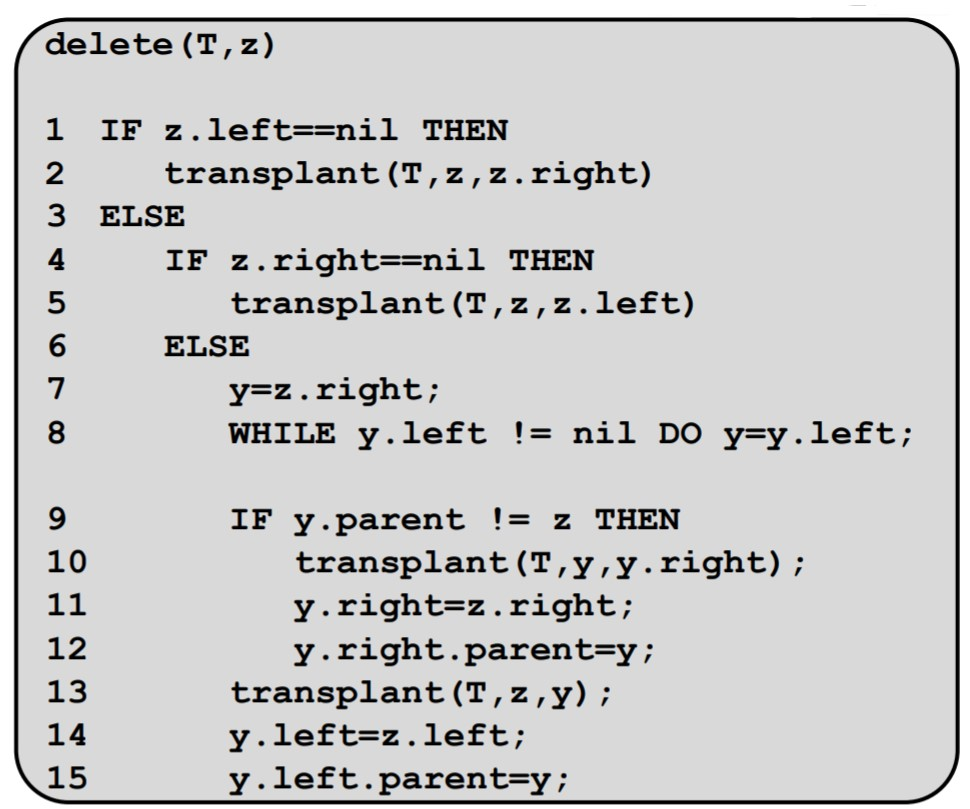
\includegraphics[scale=0.3]{BSBDeleteCode.jpg}
				\end{center}
		\end{minipage}


		\vspace{2cm}
		\begin{minipage}[t]{0.5\textwidth}
			\subsubsection{Höhe eines BST}
				\begin{itemize}
					\item Da die Laufzeit abhängig von der Höhe ist, lohnt es sich hier einen weiteren Blick drauf 
					zu werfen
					\item Im Worst Case beträgt die Laufzeit nun $\Omega(n)$, im Best Case $O(\log_{2}n)$
			\end{itemize}
		\end{minipage}
		\begin{minipage}[t]{0.45\textwidth}
			\begin{center}
				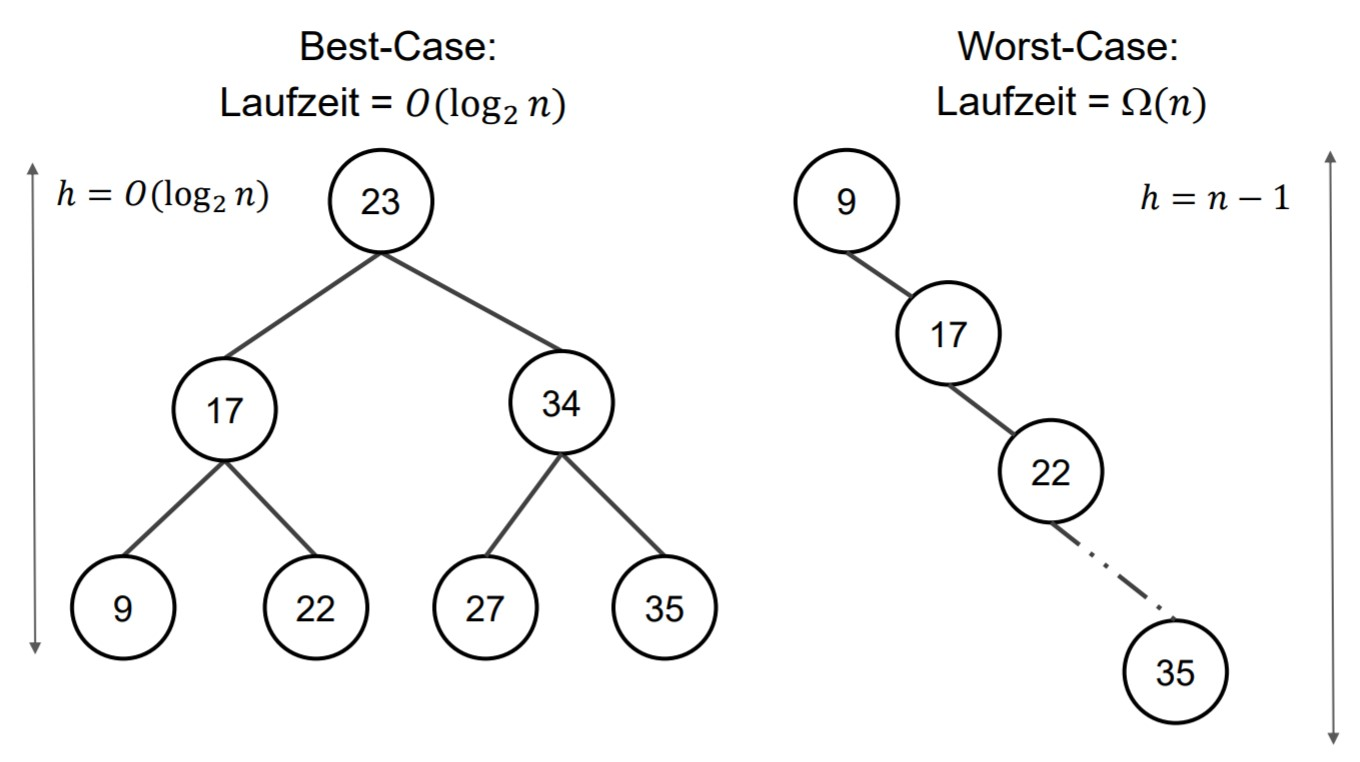
\includegraphics[scale=0.4]{BSBHoehe.jpg}
			\end{center}
		\end{minipage}


	\newpage
	\subsection{AVL Bäume}
		\begin{minipage}{0.6\textwidth}
			\subsubsection{Eigenschaften}
				\begin{itemize}
					\item Ein AVL (Adelson-Velski und Landis) Baum ist zunächst ein normaler Binärer Suchbaum
					\item Optimiert: $h \leq 2*\log n (RBT)$ vs $h \leq 1.441 * \log n (AVL/Bäume)$
				\end{itemize}
		\end{minipage}
		\hspace{1cm}
		\begin{minipage}{0.3\textwidth}
				\begin{center}
			\subsubsection{Charakteristik}
					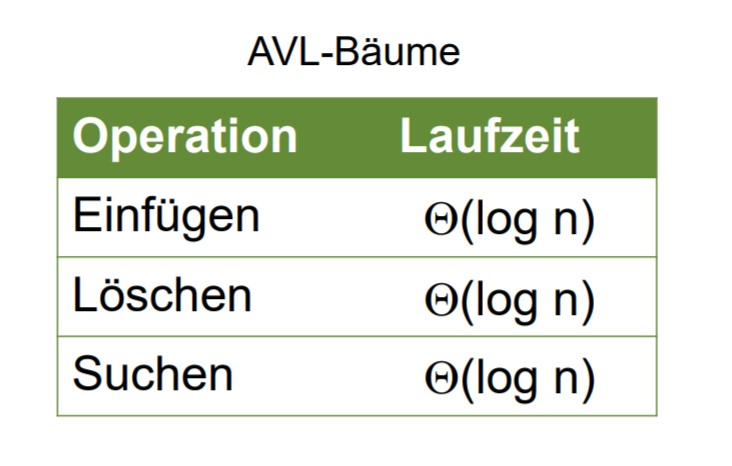
\includegraphics[scale=0.3]{AVLCharacteristic.jpg}
				\end{center}
		\end{minipage}

		\subsubsection{Definition}
			\begin{minipage}{0.65\textwidth}
				\begin{itemize}
					\item $B(x) = Höhe(rechter Teilbaum) - Höhe(linker Teilbaum)$
					\item Für alle Knoten x aus einem Baum muss $B(x) \in {-1, 0, 1}$
					\item Mit $n$ Knoten ergibt sich: $ min(n_h) = Fibonacci_{h+2} - 1$
				\end{itemize}
			\end{minipage}
			\begin{minipage}{0.2\textwidth}
				\begin{center}
					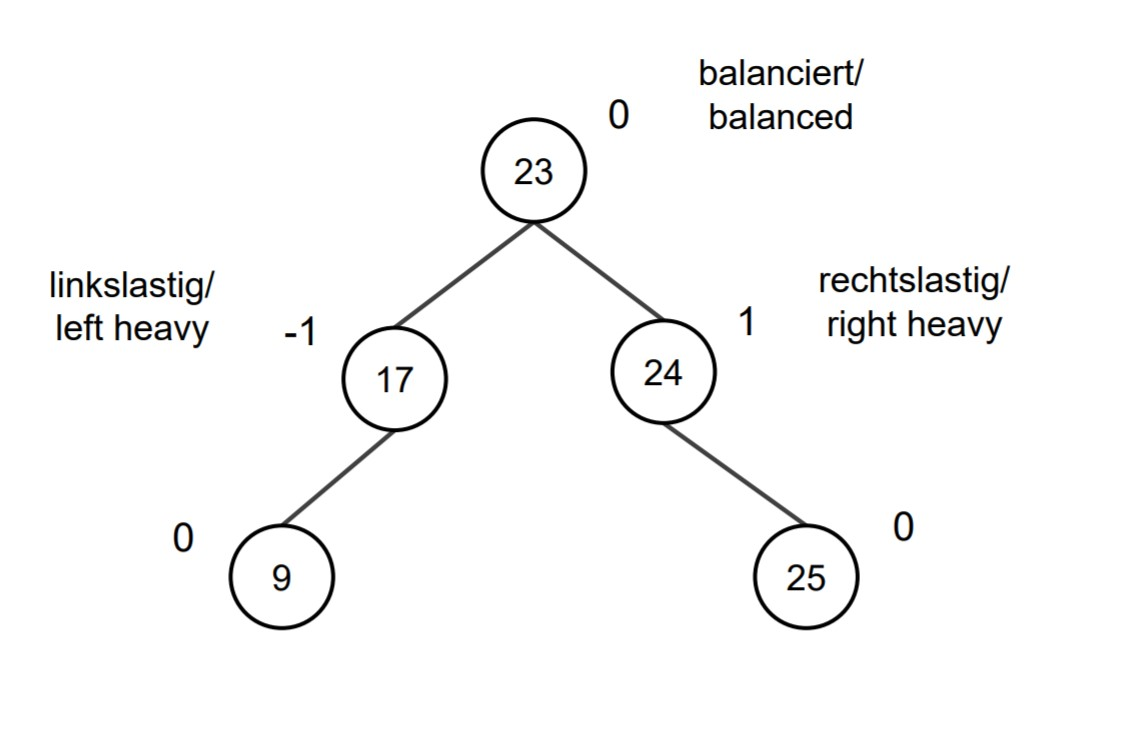
\includegraphics[scale=0.3]{AVLBeispiel.jpg}
				\end{center}
			\end{minipage}

		\subsubsection{AVL $\subset$ RBT}
			\begin{minipage}{0.6\textwidth}
				\begin{itemize}
					\item AVL-Bäume sind eine Teilmenge der Rot-Schwarz-Bäume
					\item Da ihre Teilbaumhöhe kleiner ist, als die eines RBT, lassen sich alle AVL-Bäume
						als RBT darstellen
				\end{itemize}
			\end{minipage}
			\begin{minipage}{0.35\textwidth}
				\begin{center}
					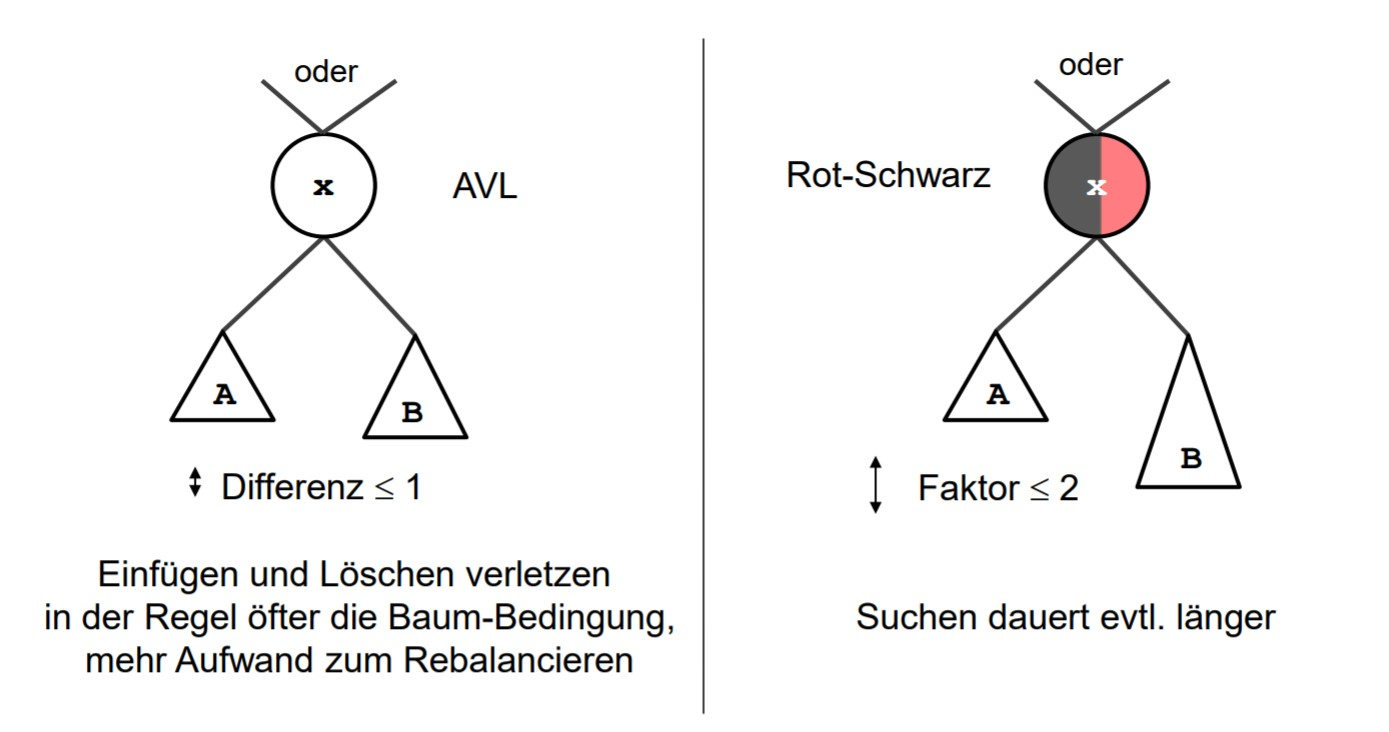
\includegraphics[scale=0.3]{AVLRBT.jpg}
				\end{center}
			\end{minipage}


		\subsubsection{Einfügen und Löschen}
			\begin{itemize}
				\item Sowohl das einfügen als auch das Löschen funktioniert gleich wie bei Binären Suchbäumen
				\item Am Ende beider Operationen kann es notwednig sein zu Rebalancieren \\
			\end{itemize}

			\noindent Einfügen - Rebalance: Fall 01:
			\noindent \paragraph{} Manchmal kann schon eine einfache Rotation das Gleichgewicht wiederherstellen.
			Da dies nicht immer der Fall ist, und die Analyse der weiteren Schritte sehr Komplex ist, 
			belassen wir es bei diesem einfachen Fall. \\
			In allen Fällen muss nur einmal Rebalanicert werden, aber es muss die zu balancierende Stelle
			gefunden werden (O(h))

			
		\subsubsection{Einfügen: Rebalancieren}
			\begin{minipage}[t]{0.5\textwidth}
				\begin{center}
					Fall 01 \\
					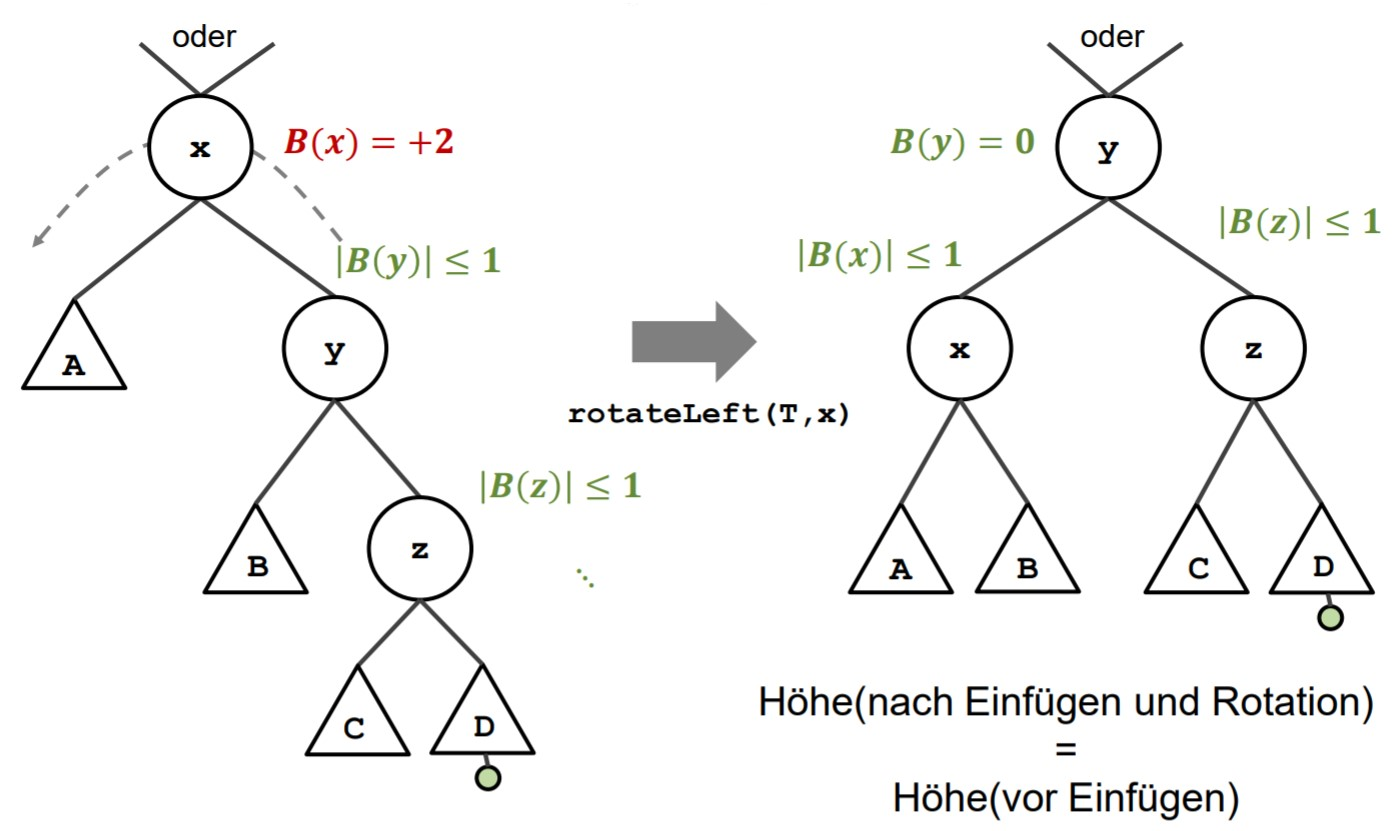
\includegraphics[scale=0.3]{AVLRebalanceCase01.jpg}
				\end{center}
			\end{minipage}
			\hfill\vline\hfill
			\begin{minipage}[t]{0.45\textwidth}
				\begin{center}
					Fall 3/4 \\
					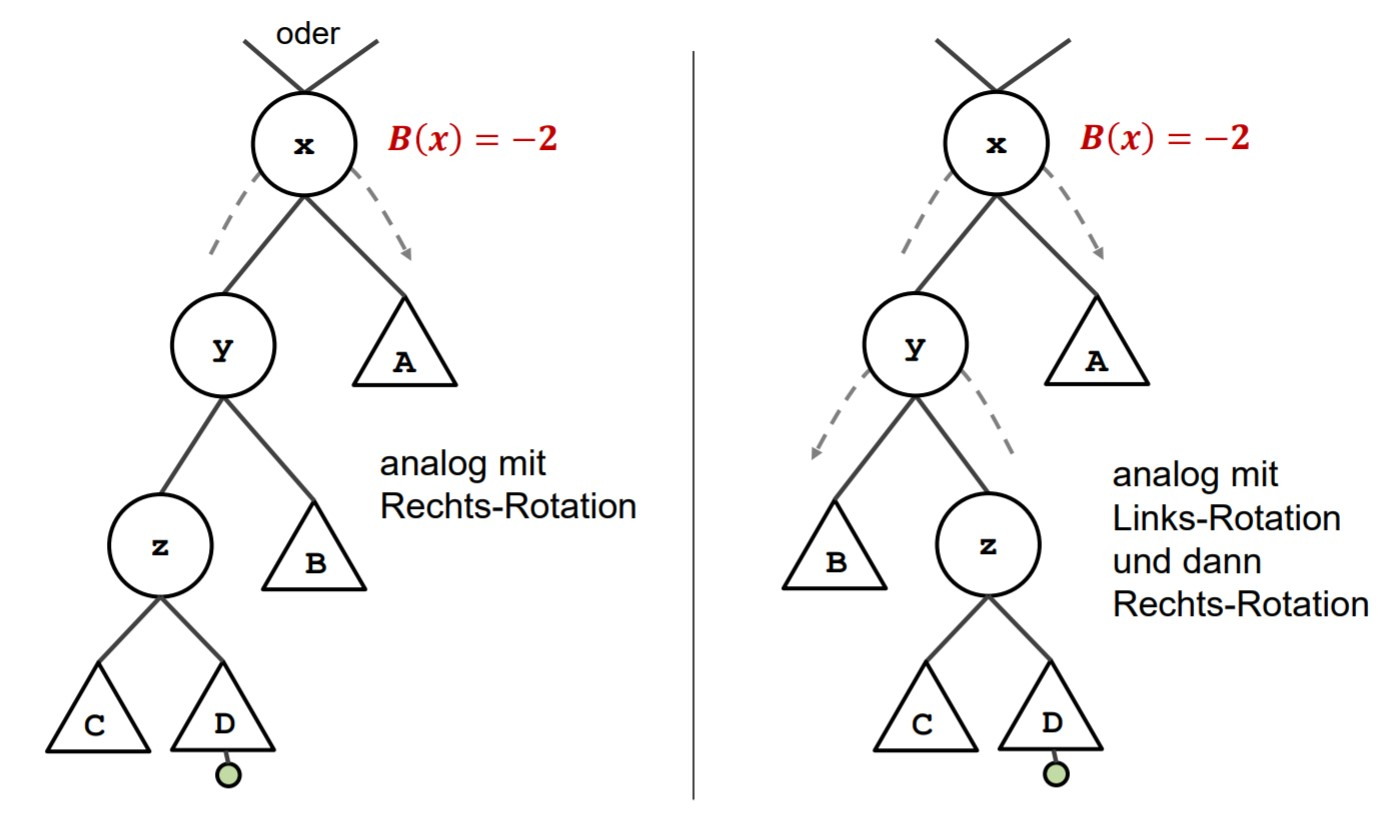
\includegraphics[scale=0.3]{AVLRebalanceCase034.jpg}
				\end{center}
			\end{minipage}
			\centerline{\noindent\makebox[0.5\linewidth]{\rule{0.9\paperwidth}{0.4pt}}}
			\begin{center}
				Fall 02 \\
				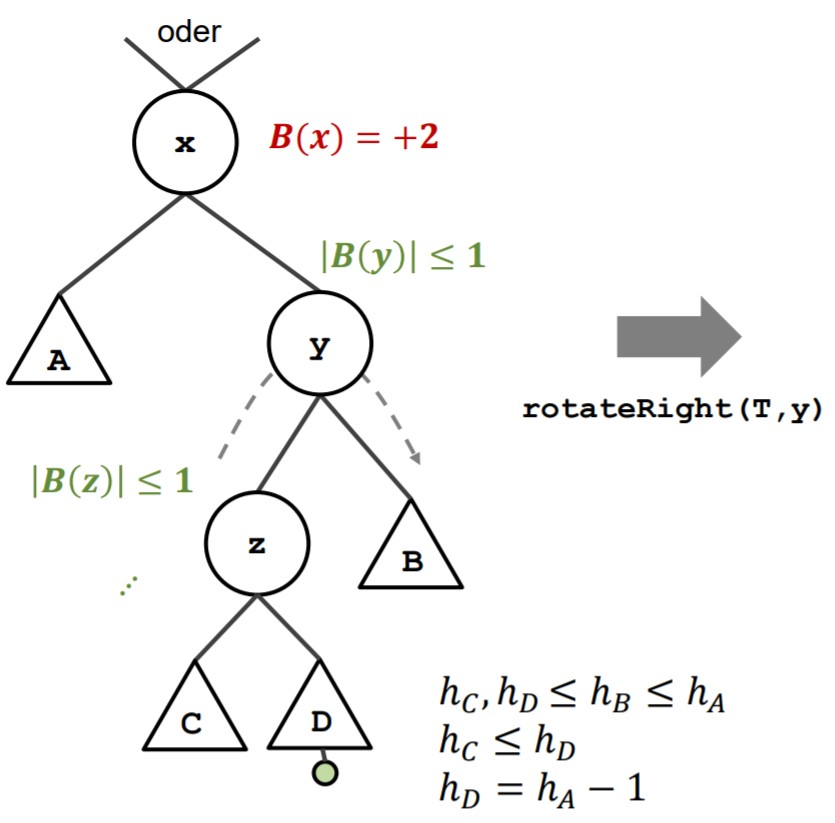
\includegraphics[scale=0.35]{AVLRebalanceCase02_1.jpg}
				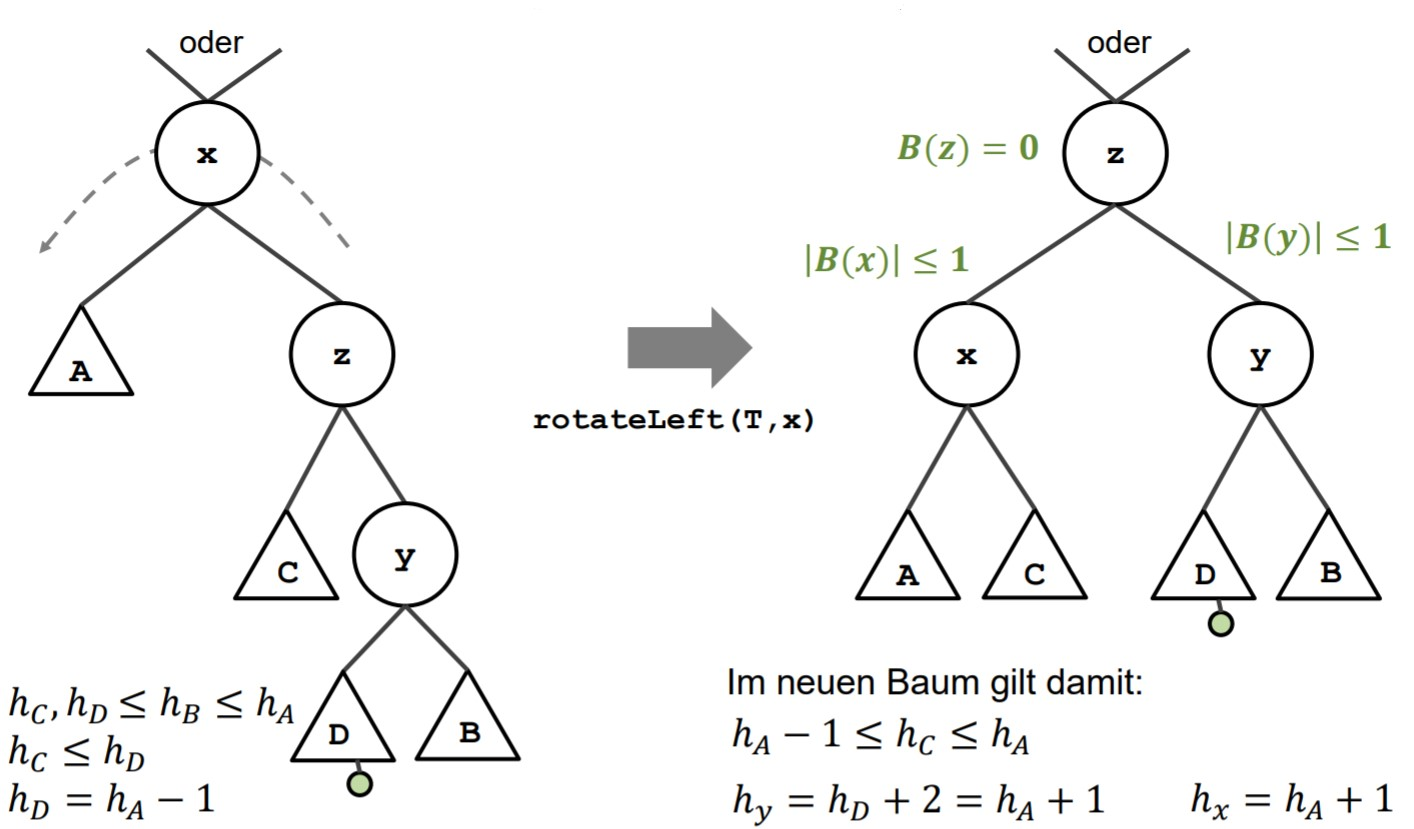
\includegraphics[scale=0.35]{AVLRebalanceCase02_2.jpg}
			\end{center}

			
	\newpage
	\subsection{Splay-Bäume}
		\subsubsection{Eigenschaften}
			\begin{itemize}
				\item Selbst organiserende Datenstruktur
				\item Beruht auf Zeitlicher Lokalität (wird ein Objekt einmal gesucht,
					wird es vermutlich in naher Zukunft erneut gesucht)
				\item Anwendungsbeispiel: SQUID - Web Cache Proxy
				\item $Splay-Bäume \subset BST$
				\item Prinziep: Spüle neu eingefügten oder gesuchten Knoten an die Wurzel
				\item In der Realität umstritten ob die Implementierung sinnvoll ist
			\end{itemize}

		\subsubsection{Einfügen und Suchen}
			\begin{itemize}
				\item Funktioniert analog zu BST, aber mit einer Splay operation
				\item Bei dieser wird ein Knoten an die Wurzel gespült
			\end{itemize}
			\begin{minipage}[t]{0.45\textwidth}
				\begin{center}
					Einfügen: \\
				\end{center}
				\begin{itemize}
					\item Nach dem Einfügen wird das Ergebnis an die Wurzel gespült
				\end{itemize}
				\begin{center}
					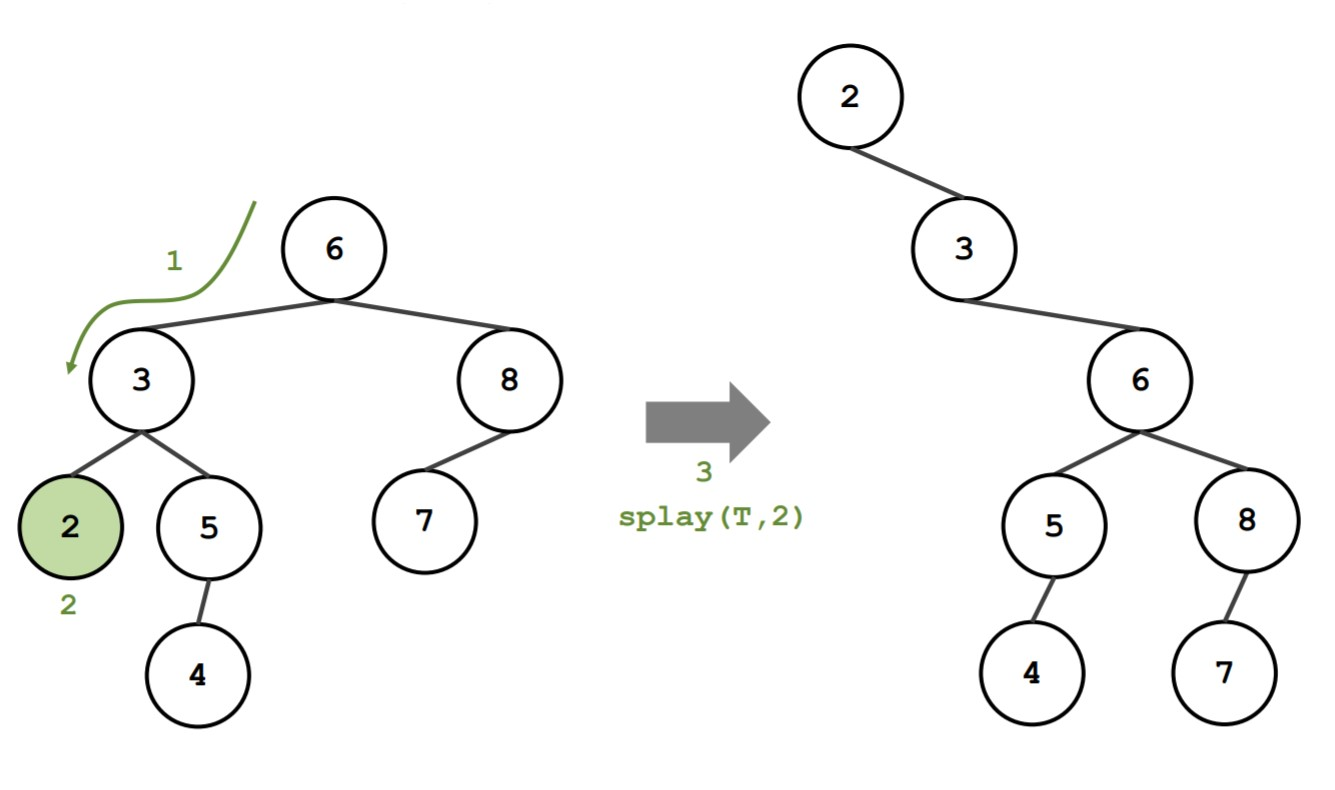
\includegraphics[scale=0.32]{SplayTreeSearch.jpg}
				\end{center}
			\end{minipage}
			\hspace{1cm}
			\begin{minipage}[t]{0.5\textwidth}
				\begin{center}
					Suchen: \\
				\end{center}
				\begin{itemize}
					\item Am Ende des Suchens wird ein eventuell gefundenes Ergebnis gespült
				\end{itemize}
				\begin{center}
					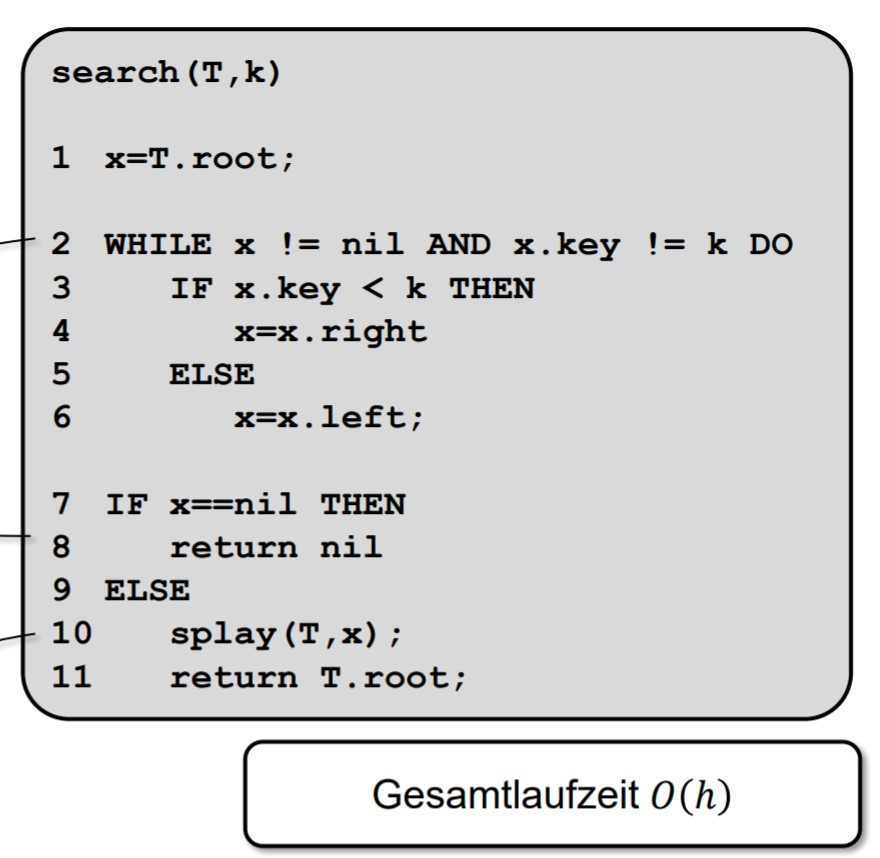
\includegraphics[scale=0.36]{SplayTreeInsert.jpg}
				\end{center}
			\end{minipage}

		\subsubsection{Splay}
			\begin{minipage}{0.55\textwidth}
				\begin{itemize}
					\item Die Spüloperation (Splay) dient dazu einen Knoten an die Wurzel zu spülen
					\item Dies dient dazu den Baum im allgemeinen ausgeglichener zu halten
					\item Gespült wird immer nach Einfügen und Suchen, sowie vor dem Löschen
					\item Das Spülen basiert dabei auf drei Unterroutinen: \\
				\end{itemize}
			\end{minipage}
			\hspace{1cm}
			\begin{minipage}{0.4\textwidth}
				\begin{center}
					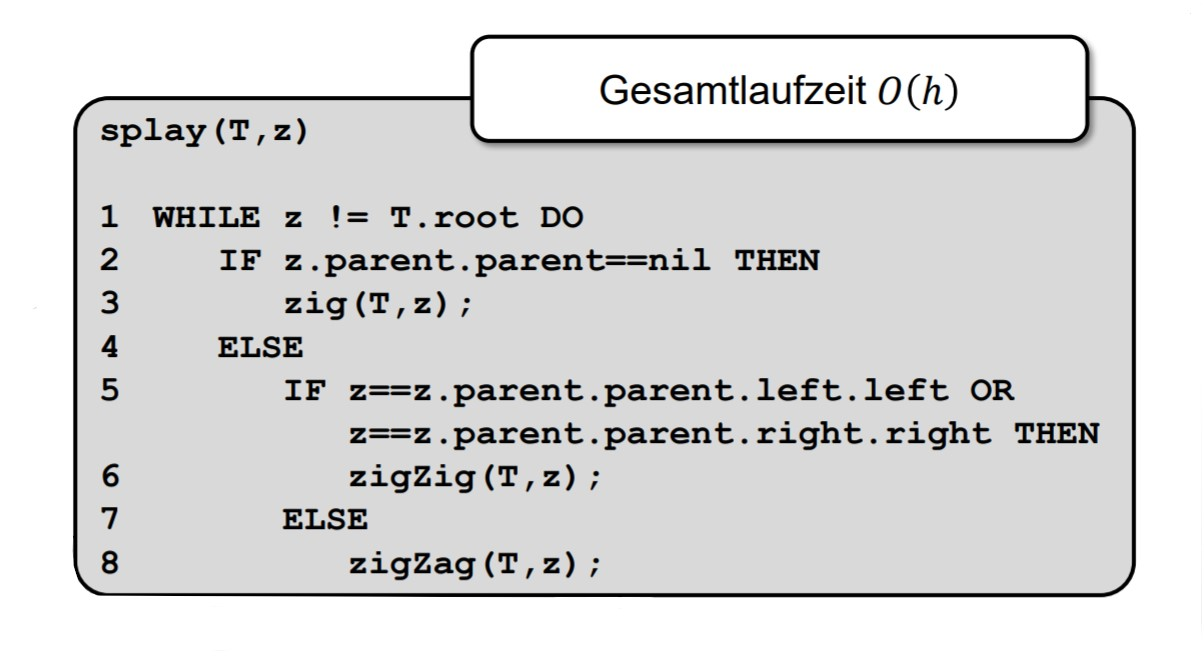
\includegraphics[scale=0.34]{SplayTreeSplay.jpg}
				\end{center}
			\end{minipage}

			\begin{center}
				ZigZag
			\end{center}
			\begin{minipage}{0.5\textwidth}
				\begin{itemize}
					\item 1. Rechtsrotation (Weg vom "Stamm") um x.parent
					\item 2. Linksrotation (Zum "Stamm") um x.parent
				\end{itemize}
			\end{minipage}
			\hspace{1cm}
			\begin{minipage}{0.45\textwidth}
				\begin{center}
					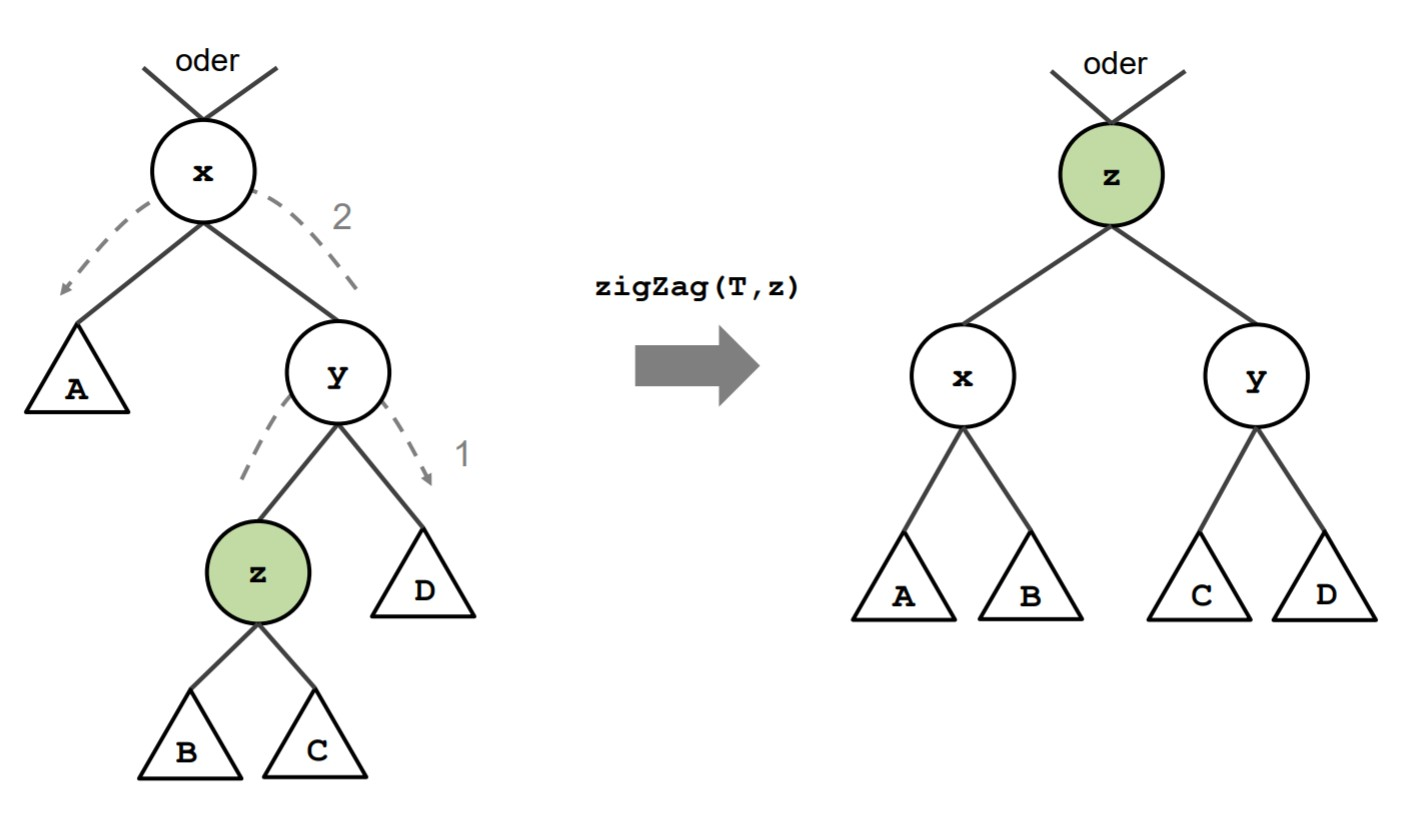
\includegraphics[scale=0.3]{SplayTreeZigZag.jpg}
				\end{center}
			\end{minipage}
			\begin{center}
				\centerline{\noindent\makebox[0.5\linewidth]{\rule{0.5\paperwidth}{0.4pt}}}
			\end{center}
			\centerline{ZigZig}
			\begin{minipage}{0.5\textwidth}
				\begin{itemize}
					\item 1. Linksrotation (Zum "Stamm") um x.parent.parent
					\item 2. Linksrotation (Zum "Stamm") um x.parent
				\end{itemize}
			\end{minipage}
			\hspace{1cm}
			\begin{minipage}{0.45\textwidth}
				\begin{center}
					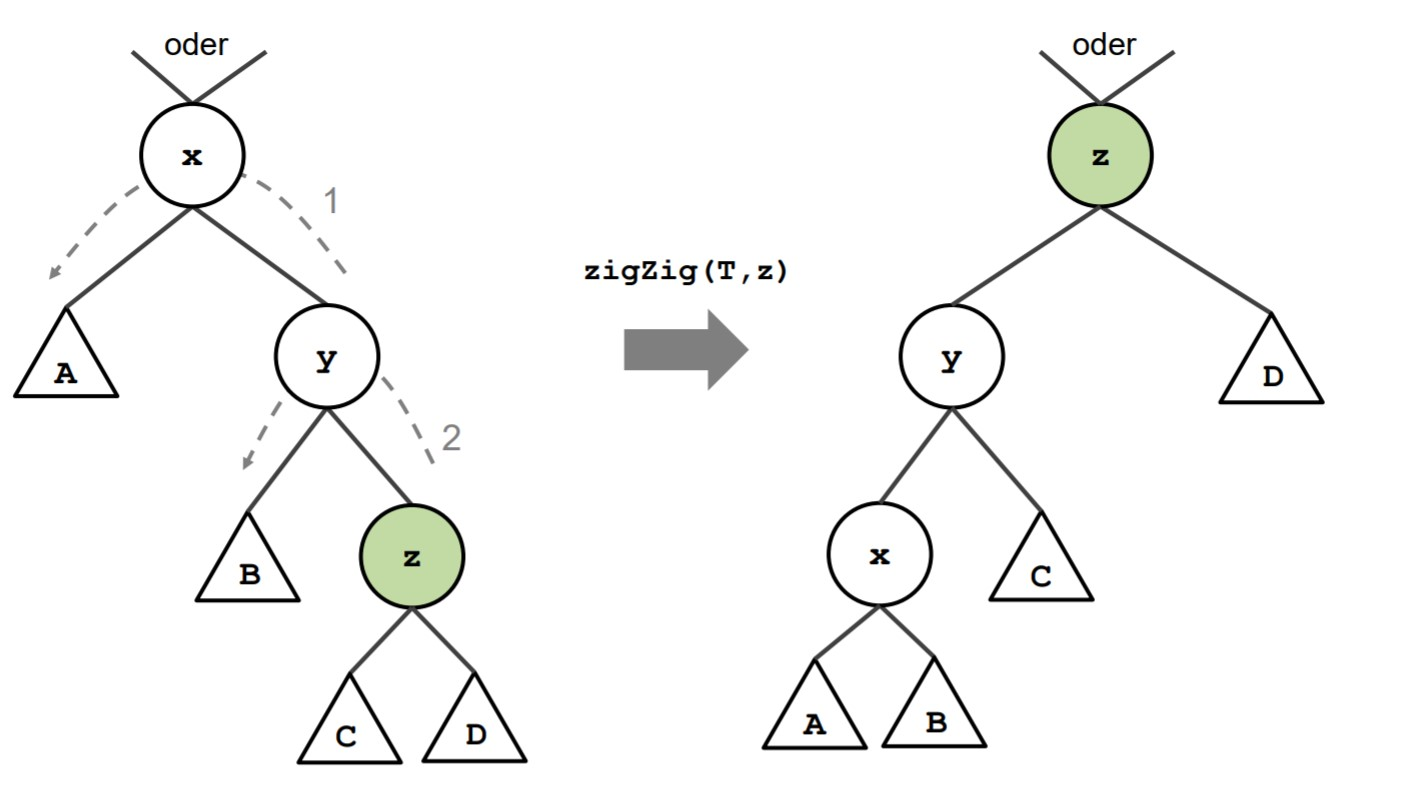
\includegraphics[scale=0.3]{SplayTreeZigZig.jpg}
				\end{center}
			\end{minipage}
			\begin{center}
				\centerline{\noindent\makebox[0.5\linewidth]{\rule{0.5\paperwidth}{0.4pt}}}
			\end{center}
			\centerline{Zig}
			\begin{minipage}{0.5\textwidth}
				\begin{itemize}
					\item 1. Linksrotation (Zum "Stamm") um x.parent
				\end{itemize}
			\end{minipage}
			\hspace{1cm}
			\begin{minipage}{0.45\textwidth}
				\begin{center}
					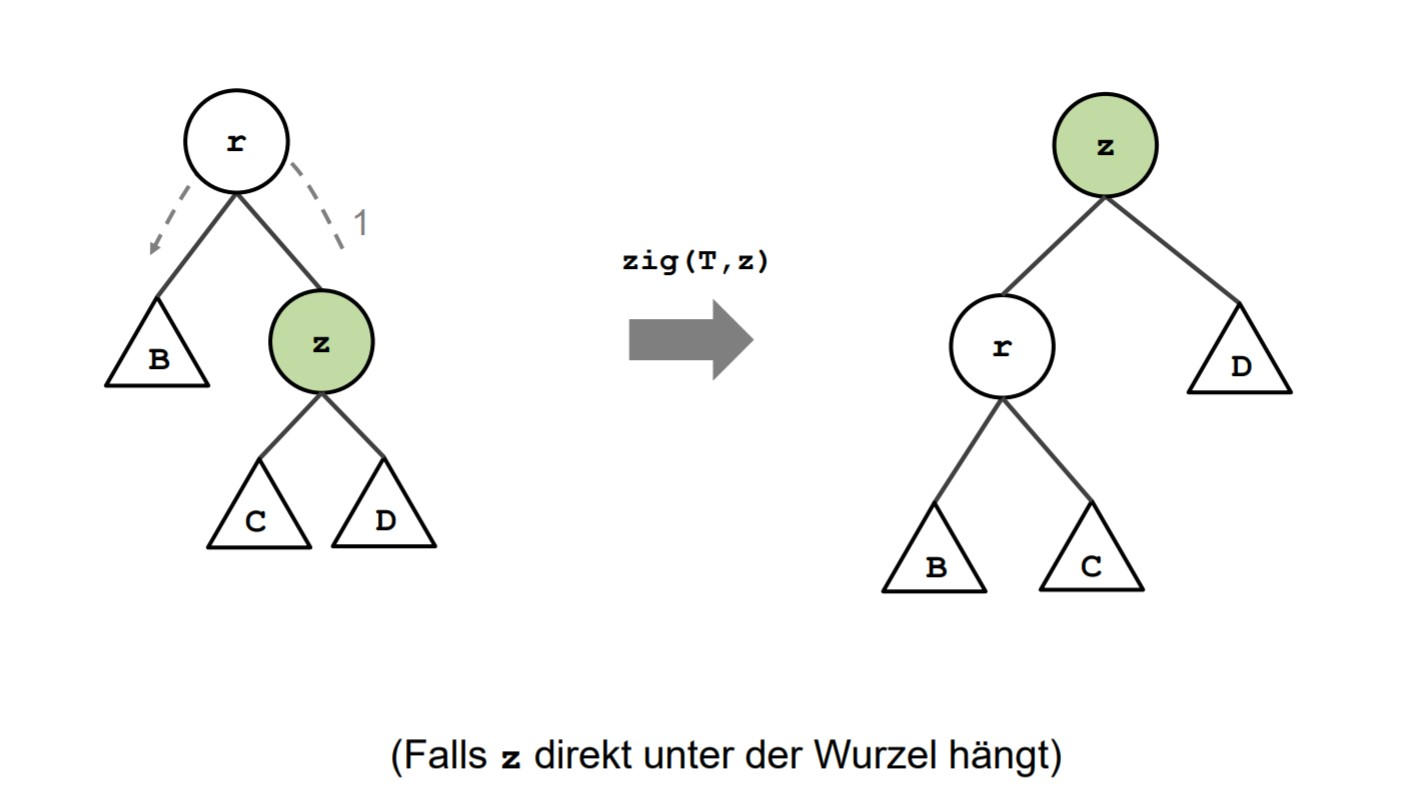
\includegraphics[scale=0.3]{SplayTreeZig.jpg}
				\end{center}
			\end{minipage}


		\subsubsection{Löschen}
			\begin{minipage}{0.5\textwidth}
				% \vspace{0.8cm}
				Schritt 1:
				\begin{itemize}
					\item Suche zu löschenden Knoten und spüle ihn an die Wurzel
				\end{itemize}

				\vspace{0.8cm}
				Schritt 2:
				\begin{itemize}
					\item Löschen von x
					\item Ist einer der resultierenden Teilbäume leer, sind wir fertig
				\end{itemize}

				\vspace{0.8cm}
				Schritt 3:
				\begin{itemize}
					\item Spüle den "grö\ss ten" Knoten $y$ in $L$ nach oben
					\item Da es mindestens der grö\ss te Wert ist, hat dieser danach 
						nur ein linkes Kind
				\end{itemize}

				\vspace{0.8cm}
				Schritt 4:
				\begin{itemize}
					\item Hänge $R$ an $y$ an
				\end{itemize}
			\end{minipage}
			\hspace{1cm}
			\begin{minipage}{0.45\textwidth}
				\begin{center}
					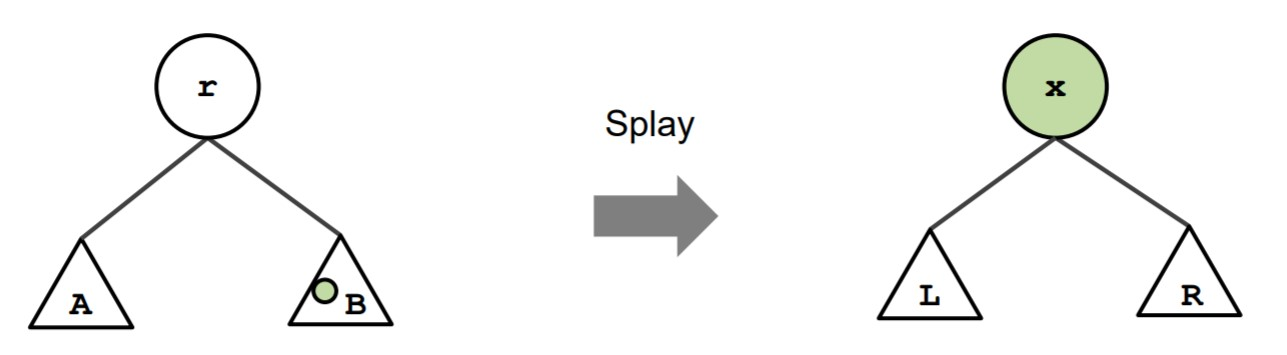
\includegraphics[scale=0.35]{SplayTreeDelete1.jpg} \\
					\vspace{2.4cm}
					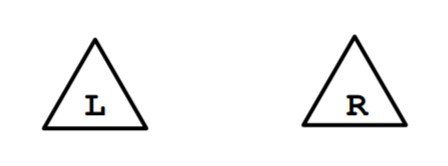
\includegraphics[scale=0.35]{SplayTreeDelete2.jpg} \\
					\vspace{2.4cm}
					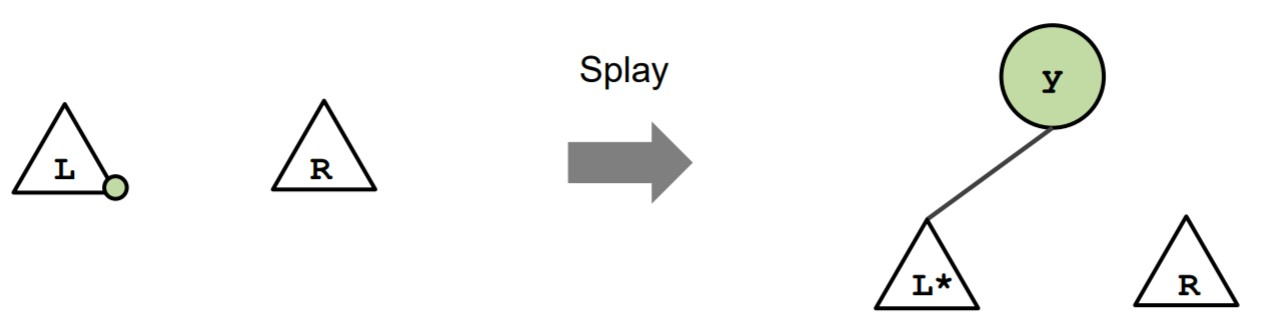
\includegraphics[scale=0.35]{SplayTreeDelete3.jpg} \\
					\vspace{0.8cm}
					\includegraphics[scale=0.35]{SplayTreeDelete4.jpg} \\
				\end{center}
			\end{minipage}
			

	\newpage
	\subsection{Binäre Max-Heaps}
		\subsubsection{Eigenschaften}
			\begin{itemize}
				\item Ein binärer Max-Heap ist ein binärer Baum (\textbf{kein Binärer Suchbaum}), der:
				\item (1) "bis auf das unterste Level vollständig und von Links gefüllt ist"
				\item (2) Für alle Knoten $\texttt{x} \neq \texttt{T.root}$ gilt, 
					$\texttt{x.parent.key} \geq \texttt{x.key}$
				\item Genauso gibt es Min-Heaps, wobei sich die Bedingung umdreht
			\end{itemize}


		\subsubsection{Heaps durch Arrays}
			\begin{minipage}{0.5\textwidth}
				\begin{itemize}
					\item Bei der Nummerierung gehen wir von oben links nach unten rechts vor
					\item Anzahl Knoten in \texttt{H} ist gleich \texttt{H.length}
					\item Duale Sichetwiese, als Pointer oder als Index:
				\end{itemize}

				\begin{center}
					\includegraphics[scale=0.4]{HeapsArrayBeziehungen.jpg}
				\end{center}
			\end{minipage}
			\begin{minipage}{0.45\textwidth}
				\begin{center}
					\includegraphics[scale=0.33]{HeapsArray.jpg}
					\includegraphics[scale=0.33]{HeapsArray2.jpg}
				\end{center}
			\end{minipage}


		\subsubsection{Einfügen}
			\begin{minipage}{0.5\textwidth}
				\begin{itemize}
					\item Wir fügen neue Knoten immer an das des Arrays ein
					\item Eventuell wird Heap Bedingung verletzt
					\item Dann Tauschen wir solange nach oben, bis dies nicht mehr der Fall ist
				\end{itemize}
			\end{minipage}
			\hspace{0.8cm}
			\begin{minipage}{0.45\textwidth}
				\begin{center}
					\includegraphics[scale=0.38]{HeapsArrayInsert.jpg}
				\end{center}
			\end{minipage}


		\subsubsection{Löschen des Maximums}
			\begin{itemize}
				\item Beim Löschen des Maximums wird das Maximum, also die Wurzel zurückgegeben
					und durch das letzte "Blatt" also das zuletzt eingefügte Element ersetzt
				\item Danach wird die Heap Bedingung mittels der Routine \texttt{heapify} wieder
					hergestellt
				\item Heapify tasucht das Element dabei immer weiter nach untern bis die Bedingung 
					wieder hergestellt ist. Dabei wird immer in den Teilbaum mit dem grö\ss eren Wert
					getauscht
			\end{itemize}

			\begin{minipage}{0.56\textwidth}
				\includegraphics[scale=0.38]{HeapArrayHeapify.jpg}
			\end{minipage}
			\begin{minipage}{0.44\textwidth}
				\includegraphics[scale=0.4]{HeapArrayExtractMax.jpg}
			\end{minipage}


		\subsubsection{Heap-Konstruktion aus Array}
			\begin{itemize}
				\item Aus einem Array lässt sich realtiv einfach ein Heap erzeugen
				\item Da Einelementige Heaps trivialerweise alle Heap Bedingungen erfüllen
					müssen wir die Bedingung nur bei allen Elementen außer den Blättern wieder
					herstellen
				\item Die Blätter Indices ergeben sich: \includegraphics[scale=0.4]{HeapArrayLeafIndex.jpg}
			\end{itemize}

			\begin{center}
				\includegraphics[scale=0.4]{HeapArrayBuildHeap.jpg}
			\end{center}

		
		\subsubsection{Heap-Sort}
			\begin{minipage}{0.5\textwidth}
				\begin{itemize}
					\item Mittels eines Heapes lässt sich auch sortieren
					\item Dabei wird der Heap z.B. erst aus einem Array gebildet, und danach
						werden alle Elemente wieder ins Array eingefügt
					\item (gibt Array in absteigender Reihenfolge zurück)
				\end{itemize}
			\end{minipage}
			\hspace{0.8cm}
			\begin{minipage}{0.45\textwidth}
				\begin{center}
					\includegraphics[scale=0.4]{HeapSort.jpg}
				\end{center}
			\end{minipage}


	\newpage
	\subsection{B-Bäume}
		\subsubsection{Eigenschaften}
			\begin{itemize}
				\item B könnte für Balanced, Bayer-McCreight oder für Boeing stehen
				\item Ein B-Baum (vom Grad $t$) ist ein Baum, bei dem
				\item (1) jeder Knoten (au\ss er der Wurzel) mindestend $t - 1$, und maximal $2t - 1$
					Werte hat
				\item (2) die werte innnerhabl eines Knoten sind aufsteigend sortiert
				\item (3) die Blätte ralle die gleiche Höhe haben
				\item (4) jeder innere Knoten mit $n$ Werten und $n + 1$ Kindern, so dass für alle
					Werte $k_j$ aus dem $j-$ten Kind gilt: $k_0 \leq key[0] \leq k_1 \leq \dots \leq k_{n-1} \leq key[n-1] \leq k_n$
			\end{itemize}


		\subsubsection{Höhe B-Baum}
			\begin{minipage}{0.5\textwidth}
				\begin{itemize}
					\item Für grö\ss ere Werte ist ein B-Baum also flacher als (vollständiger) Binärbaum
				\end{itemize}

				\begin{center}
					\includegraphics[scale=0.4]{BBaumHoehe2.jpg}
				\end{center}
			\end{minipage}
			\begin{minipage}{0.45\textwidth}
				\begin{center}
					\includegraphics[scale=0.4]{BBaumHoehe.jpg}
				\end{center}
			\end{minipage}
			
		
		\subsubsection{Anwendung}
			\begin{itemize}
				\item B-Bäume werden dort verwendet wo man im allgemeinen öfter auf ganze Blöcke 
					von Daten zugreifen möchte
				\item Beispiel: Festplatten, hier wird Blockweise auf die Werte zugegriffen um gleichzeitig
					mehrere Indices zu bekommen
				\item Beispiel: Auch die MySQL Datenbank nutzt B-Baume zur Speicherung von manchen Indices
			\end{itemize}


		\subsubsection{Baumkunde}
			\begin{center}
				\includegraphics[scale=0.35]{BBaumBaumkunde.jpg}
			\end{center}


		\subsubsection{Suchen}
			\begin{minipage}{0.5\textwidth}
				\begin{itemize}
					\item Das Suchen funktioniert ähnlich wie bei Binären Suchbäumen
				\end{itemize}
			\end{minipage}
			\begin{minipage}{0.45\textwidth}
				\begin{center}
					\includegraphics[scale=0.4]{BBaumSearch.jpg}
				\end{center}
			\end{minipage}


		\subsubsection{Einfügen}
			\begin{itemize}
				\item Zuerst wird die Position gesucht an der eingefügt werden muss
				\item Einfügen erfolgt zunächst immer im Blatt
				\item Hat das Blatt nach Einfügen immer noch weniger als $2t - 1$ Werte sind wir fertig
				\item Hat der Knoten schon maximale Werte, muss der Knoten gesplittet werden
				\item Beim Splitten wird der Mittlere Wert in den Eltern Knoten eingefügt
				\item Eventuell muss hier rekursiv nach oben gegangen werden
			\end{itemize}

			\begin{minipage}[t]{0.5\textwidth}
				\begin{center}
					Einfügen und Splitten \\
					\includegraphics[scale=0.35]{BBaumInsert}
				\end{center}
			\end{minipage}
			\hspace{1cm}
			\begin{minipage}[t]{0.45\textwidth}
				\begin{center}
					\includegraphics[scale=0.35]{BBaumInsertRoot.jpg}
				\end{center}
			\end{minipage}


		\subsubsection{Suchen, dann Splitte vs Suchen und Splitte}
			\begin{minipage}[t]{0.5\textwidth}
				\begin{itemize}
					\item Beim Einfügen wird erst gesucht, und danach wird Gesplittet
					\item Um das zweifache traversieren durch den Baum zu vermeiden kann man 
						auch anders vorgehen
					\item bei deiser Strategie wird beim suchen gleichzeitig gesplittet
				\end{itemize}
			\end{minipage}
			\hspace{1cm}
			\begin{minipage}[t]{0.45\textwidth}
				\begin{center}
					\includegraphics[scale=0.35]{BBaumInsertWithSplit.jpg}
				\end{center}
			\end{minipage}


		\subsubsection{Löschen}
			Löschen im Blatt: \\ \\
			\begin{minipage}{0.6\textwidth}
				\begin{itemize}
					\item Wird in einem Blatt gelöscht, dass zu wenig Knoten hat, 
						gibt es zwei Möglichkeiten
					\item (1 Rotieren) Hat der Nachbarknote noch ausreichen Elemente,
						dann kann rotiert werden
					\item (2 Verschmelzen) Hat kein Nachbarknoten ausreichend Elemente zum Rotieren,
						müssen wir Verschmelzen
					\item Dies läuft daraus hinaus, dass der Eltern Knoten ein Element weniger hat, 
						und zwei Kindknoten zu einem Verschmelzen
					\item Hierbei kann es passieren, dass dabei die Balance im Elterknoten gestört
						ist. Dies muss rekursiv behoben werden
				\end{itemize}
			\end{minipage}
			\hspace{0.5cm}
			\begin{minipage}{0.35\textwidth}
				\begin{center}
					\hspace{0.3cm} Rotieren \hspace{1.1cm} Verschmelzen \\
					\includegraphics[scale=0.3]{BBaumLöschenRotieren.jpg}
					\includegraphics[scale=0.3]{BBaumLöschenVerschmelzen.jpg}
				\end{center}
			\end{minipage}
			\mbox{} \\ \\ \\

			\noindent Löschen im inneren Knoten: \\ \\
			\begin{minipage}{0.6\textwidth}
				\begin{itemize}
					\item Wird in einem inneren Knoten gelöscht gibt es zwei Möglichkeiten
					\item (1 Verschieben) Wenn einer der beiden Kindknoten mehr als $t-1$ Werte hat,
						kann der gelöschte Wert ersetzt werden, mit dem
						\begin{itemize}
							\item grö\ss ten Wert des linken Kindes
							\item kleinsten Wert des rechten Kindes
						\end{itemize}
					\item (2 Verschmelzen) Wenn beide Kindknoten jeweils zu wenig Elemente
						haben (also $t-1$) werden diese beiden Knoten verschmolzen
					\item Auch hierbei kann es passieren, dass der Elternknoten zu wenige Elemente 
						hat, hier wird dann rekursiv vorgegangen

				\end{itemize}
			\end{minipage}
			\hspace{0.5cm}
			\begin{minipage}{0.35\textwidth}
				\begin{center}
					Verschieben \hspace{1cm} Verschmelzen
					\includegraphics[scale=0.3]{BBaumLöschenVerschieben.jpg}
					\includegraphics[scale=0.3]{BBaumLöschenVerschmelzen02.jpg}
				\end{center}
			\end{minipage}
			\mbox{} \\ \\ \\
		

		\begin{minipage}[t]{0.5\textwidth}
			\subsubsection{Löschen und Splitte}
				\begin{center}
					\includegraphics[scale=0.4]{BBaumLöschenCode.jpg}
				\end{center}
		\end{minipage}
		\begin{minipage}[t]{0.45\textwidth}
			\subsubsection{Cahrakteristik}
				\begin{center}
					\includegraphics[scale=0.4]{BBaumCharakteristik.jpg}
				\end{center}
		\end{minipage}


	\newpage
	\subsection{Skip-Lists}
		\begin{minipage}[t]{0.55\textwidth}
			\subsubsection{Eigenschaften}
				\begin{itemize}
					\item Skip Listen sind ein Beispiel für Randomisierte Datenstrukturen
					\item Dies bedeutet: Verhalten hängt von zufälligen Entscheidungen
						der Datenstruktur ab
					\item Gegensatz: deterministische Datenstrukturen - Verhalten für 
						identische Eingaben immer gleich \\
				\end{itemize}

			\subsubsection{Anwendungen}
				\begin{itemize}
					\item Einfügen / Löschen unterstützen parallele Verarbeitung (z.B. Multi-Core-Systeme),
						da nur sehr lokale Änderungen (im Vergleich zum Re-Balancieren bei Bäumen)
					\item Dafür logarithmische Laufzeit nur um Durchschnitt
				\end{itemize}
		\end{minipage}
		\hspace{1cm}
		\begin{minipage}[t]{0.4\textwidth}
			\begin{center}
				\subsubsection{Charakteristik}
					\includegraphics[scale=0.35]{SkipListsCharakteristik.jpg}
					\includegraphics[scale=0.35]{SkipListsCharakteristikDurchschnitt.jpg}
			\end{center}
		\end{minipage}


		\subsubsection{Idee von Skip-Listen}
			\begin{itemize}
				\item Eine Skip Liste besteht zunächst aus einem Array, welches erstes Element auf $-\infty$
					gesetzt
			\end{itemize}

			\begin{minipage}{0.5\textwidth}
				\begin{itemize}
					\item Darüber hinaus gibt es eine Express-Liste
						\begin{itemize}
							\item Eine Express-Liste wird mit einigen Elementen der Skip-Liste gefüllt
						\end{itemize}
					\item Es werden zusätzliche Zeiger benötigt $\Rightarrow$
				\end{itemize}
			\end{minipage}
			\hspace{1.5cm}
			\begin{minipage}{0.45\textwidth}
				\begin{center}
					\includegraphics[scale=0.36]{SkipListsPointer.jpg}
				\end{center}
			\end{minipage}

		
		\subsubsection{Suchen mittels Express-Listen}
			\begin{itemize}
				\item Beginnend in der Express-Liste: Element gefunden? $\rightarrow$ Element ausgeben
				\item Nächstes Element in Express-Liste kleiner gleich gesuchtes Element? $\rightarrow$ Weiter nach Rechts
				\item Nächstes Element in Express-Liste gr\ss er als gesuchtes Element? $\rightarrow$ Nach unten in nächste Liste
			\end{itemize}

			\begin{minipage}{0.5\textwidth}
				\begin{center}
					\includegraphics[scale=0.35]{SkipListsSearch.jpg}
				\end{center}
			\end{minipage}
			\begin{minipage}{0.45\textwidth}
				\begin{center}
					\includegraphics[scale=0.35]{SkipListsSearchCode.jpg}
				\end{center}
			\end{minipage}


		\subsubsection{Verbesserung}
			\begin{minipage}{0.5\textwidth}
				\begin{itemize}
					\item Express-Liste ist wieder eine Skip-Liste
					\item Beispiel: jede Express-Liste hat die Hälfte der Elemente der vorherigen Liste \\
						ergibt $\frac{n}{2} + \frac{n}{4} + \dots + 2 + 1 \leq n$ zusätzliche Elemente
				\end{itemize}
			\end{minipage}
			\hspace{1cm}
			\begin{minipage}{0.45\textwidth}
				\begin{center}
					\includegraphics[scale=0.35]{SkipListsVerbesserung.jpg}
				\end{center}
			\end{minipage}


		\subsubsection{Auswahl der Elemente für Express-Liste}
			\begin{itemize}
				\item Idee: Wähle jedes Element aus Liste mit Wahrscheinlichkeit
					$p$ (z.B. $p=\frac{1}{2}$) für übergeordnete Liste
				\item Wie viele Elemente gibt es auf den jeweiligen Ebenen?
			\end{itemize}


		\begin{minipage}[t]{0.5\textwidth}
			\subsubsection{Linearität des Erwartungsert}
			\includegraphics[scale=0.3]{SkipListsLinearität01.jpg}
		\end{minipage}
		\begin{minipage}[t]{0.45\textwidth}
			\subsubsection{Erwartungswert geometrisch verteilter Zufallsvariablen}
			\begin{center}
				\includegraphics[scale=0.3]{SkipListsZufallsvariablen.jpg}
			\end{center}
		\end{minipage}


		\subsubsection{Durchschnittliche Laufzeit für Suchen}
			\begin{itemize}
				\item Im schlimmsten Fall endet unsere Suche erst auf der untersten Liste
				\item Im Durchschnitt machen wir nur $\frac{1}{p}$ Schritte auf jeder Ebene, 
					bevor wir eine Ebene nach oben gegangen sind
				\item Wenn die Skip-Liste die Höhe $h$ hat, brauchen wir also im Durchschnitt \\
					$\frac{1}{p} + \frac{1}{p} + \dots + \frac{1}{p} = \frac{h}{p} = O(h) = O(\log n)$
			\end{itemize}


		\subsubsection{Einfügen}
			\begin{minipage}{0.5\textwidth}
				\begin{itemize}
					\item Beim einfügen wird als erstes die richtige Stelle gesucht werden
					\item Dort wird das Element dann in die Ursprüngliche Liste eingefügt
					\item Danach wird das Element mit der Wahrscheinlichkeit $p$ in die Liste
						obendrüber eingefügt
				\end{itemize}
			\end{minipage}
			\hspace{1cm}
			\begin{minipage}{0.45\textwidth}
				\begin{center}
					\includegraphics[scale=0.35]{SkipListsInsert.jpg}
				\end{center}
			\end{minipage}


		\subsubsection{Löschen}
			\begin{minipage}{0.5\textwidth}
				\begin{itemize}
					\item Entfernen eines Elementes funktioniert analog wie zu LinkedLists
					\item Nachdem das Element gefunden ist, müssen alle Zeiger umgeschrieben werden
				\end{itemize}			
			\end{minipage}
			\hspace{1cm}
			\begin{minipage}{0.45\textwidth}
				\begin{center}
					\includegraphics[scale=0.3]{SkipListsDelete.jpg}
				\end{center}
			\end{minipage}


	\newpage
	\subsection{Hash-Tables}
		\begin{minipage}[t]{0.65\textwidth}
			\subsubsection{Eigenschaften}
				\begin{itemize}
					\item Hashtables sind ein Beispiel für Randomisierte Datenstrukturen
					\item Hashtables sind eine gute Datenstrukturen zum Suchen und Einfügen
					\item Allerdings kann nicht auf Nachbarelemente zugegriffen werden, und die Elemente
						sind nicht sortiert
					\item Anwendung: Zum Beispiel bei SQL mittels Hash Indices, um Daten schneller zu ermitteln
				\end{itemize}
		\end{minipage}
		\hspace{0.5cm}
		\begin{minipage}[t]{0.3\textwidth}
			\begin{center}
				\subsubsection{Charakteristik}
					\includegraphics[scale=0.4]{HashtablesCharakterisitk.jpg}
			\end{center}
		\end{minipage}


		\subsubsection{Idee von Hashtables}
			\begin{minipage}{0.6\textwidth}
				\begin{itemize}
					\item Eine Hashfunktion kann als Array dargestellt werden
					\item Die Menge an Daten wird mittels einer Hashfunktion einsortiert
					\item Jeder Wert wird durch die Hashfunktion gemapped, und der daraus resultierende
						Wert ist der neue Arrayindex des Elements
					\item Damit keine Kollisionen auftreteten, sollte die Hashfunktionen "gut verteilt" sein
				\end{itemize}
			\end{minipage}
			\hspace{0.5cm}
			\begin{minipage}{0.35\textwidth}
				\begin{center}
					\includegraphics[scale=0.3]{HashtablesIdee.jpg}
				\end{center}
			\end{minipage}


		\subsubsection{Suchen und Löschen}
			\begin{minipage}{0.6\textwidth}
				\begin{itemize}
					\item Beim Suchen wird das gesuchte Element mit der Hashfunktion gemapped
					\item Befindet sich das Element in der Hashtable, ist es der zurückgegebnen Stell zu finden
					\item Beim Löschen wird das Element als erstes gesucht, und falls vorhanden gelöscht
				\end{itemize}
			\end{minipage}
			\begin{minipage}{0.35\textwidth}
				\begin{center}
					\includegraphics[scale=0.33]{HashtablesSearchDelete.jpg}
				\end{center}
			\end{minipage}
			

		\subsubsection{Kollisionsauflösung}
			\begin{itemize}
				\item Wird ein Element eingefügt kann an der Stelle schon ein Element sein 
					(dies sollte durch eine gute Hashfunktion verhindert werden)
				\item Sollte es doch dazu kommen, dass mehrere Elemente von der Hashfunktionen die
					selbe Position zugewiesen bekommen, dann gibt es mehrere Arten damit umzugehen
				\item Ein Möglichkeit ist das Erstellen von LinkedLists an den Stellen der Hashtable
			\end{itemize}

			\begin{center}
				Einfügen \hspace{8cm} LinkedLists \\
				\includegraphics[scale=0.3]{HashtablesKollision.jpg} \hspace{1cm}
				\includegraphics[scale=0.3]{HashtablesLinkedList.jpg}
			\end{center}


		\subsubsection{Hashtables mit Verketteten Listen: Laufzeit}
			\begin{itemize}
				\item Bei uniform und unabhängig verteilten Hashwerten benötigten Suchen und Löschen
					im Durchschnitt $\Theta(\frac{n}{T.length})$ viele Schritte. Einfügen benötigt
					im Worst-Case $\Theta(1)$ viele Schritte.
				\item Wählt man $T.length \approx n$ ergibt sich also konstante Laufzeit (im Durchschnitt)
			\end{itemize}


		\subsubsection{Hashfunktion}
			\begin{minipage}{0.5\textwidth}
				\begin{itemize}
					\item Eine "gute" Hashfunktion verteilt alle Werte möglichst gleichmä\ss ig 
						auf den Indexbereich das Arrays ab
					\item Eine möglichkeit ist die Universelle Hashfunktion (nebenstehend)
					\item Diese Funktion verteilt sehr gut, und jedes Element wird mit der Wahrscheinlichkeit
						$\frac{1}{p}$ getroffen
					\item Zwei Werte treffen mit einer Wahrscheinlichkeit von $\frac{1}{p^2}$ aufeinander \\
				\end{itemize}
			\end{minipage}
			\hspace{1cm}
			\begin{minipage}{0.45\textwidth}
				\begin{center}
					\includegraphics[scale=0.3]{HashtablesHashfunction01.jpg}
				\end{center}
			\end{minipage}
			\begin{itemize}
				\item Eine andere Möglichkeit sind Kryptographische Hashfunktionen wie MD5 und SHA-1 an
				(diese werden heute nicht mehr verwendet sondern ihre Nachfolger SHA-2, SHA-3)
				\item Dafür setzt man $h(x) = MD5(x) \mod T.length$
			\end{itemize}


		\subsubsection{Hashtables vs Bäume}
			\begin{itemize}
				\item In Hashtables lassen sich nur Suchen nach bestimmten Werten durchführen
				\item Um auf Nachbarwrte zuzugreifen, muss eine neue Hashfunktion berechnet werden
				\item Bei Bäumen oder anderen Datenstrukturen lassen sich schnell ganze Bereiche absuchen
				\item Desweiteren muss die Hashtable immer grö\ss er sein als die Anzahl der Elemente (in Java empholen 0.75 loadfactor)
			\end{itemize}


	\newpage
	\subsection{Bloom-Filter}
		\begin{minipage}[t]{0.45\textwidth}
			\subsubsection{Eigenschaften}
				\begin{itemize}
					\item Bloo-Filter sind ein weiteres Beispiel für Randomisierte Datenstrukturen
					\item ''Speicherschonende Wörterbücher mit kleinem Fehler''
				\end{itemize}
		\end{minipage}
		\hspace{0.5cm}
		\begin{minipage}[t]{0.5\textwidth}
			\subsubsection{Beispiel: Schlechte Passwörter}
				\begin{itemize}
					\item Um schlechte Passwörter zu vermeiden werden Bloomfilter verwendet
					\item Die Passwörter werden offline gespeichert, und online wird geprüft ob sie
						ein ''schlechtes'' Wort sein
				\end{itemize}
		\end{minipage}


		\subsubsection{Anwendung Bloom-Filter}
			\begin{itemize}
				\item NoSQL-Datenbanken: Abfrage für nicht-vorhandene Elemente verhindern
				\item Bitcoin: Prüfen von Transaktionen ohne gesamte Daten zu laden
				\item Früher auch Chrome-Browser: Erkennen schädlicher Websiten
			\end{itemize}


		\subsubsection{Bloom-Filter: Erstellen}
			\begin{minipage}{0.65\textwidth}
				\begin{itemize}
					\item Gegeben:
						\begin{itemize}
							\item $n$ Elemente $x_0 , \dots , x_{n-1}$ beliebiger Komplexität
							\item $m$ Bits Speicher , üblicherweise in einem Bit-Array
							\item $k$ ''gute'' Hash-Funktionen $H_0 , \dots , H_{k-1}$ mit Bildbereich $0,1,\dots,m-1$
						\end{itemize}
				\end{itemize}				
			\end{minipage}
			\begin{minipage}{0.45\textwidth}
				\begin{center}
					\includegraphics[scale=0.35]{BloomFilterEmpfohleneWerte.jpg}
				\end{center}
			\end{minipage}
			\begin{itemize}
				\item 1. Initialisiere Array mit 0-Einträgen
				\item 2. Schreibe für jedes Element in jede Bit-Position 
					$H_0 (x_j),\dots, H_{k-1}(x_j)$ eine 1
					\item Eventuell werden dabie Werte erneut auf 1 gesetzt	
			\end{itemize}
					
			\begin{center}
				\includegraphics[scale=0.35]{BloomFilterEinfügenCode.jpg}
				\includegraphics[scale=0.4]{BloomFilterEinfügen}
			\end{center}

			
		\subsubsection{Suchen}
			\begin{itemize}
				\item gib an, dass $y$ im Wörterbuch, wenn genau alle $k$ Einträge für $y$ in BF=1 sind
			\end{itemize}

			\begin{center}
				\includegraphics[scale=0.35]{BloomFilterSuchenCode.jpg}
				\includegraphics[scale=0.4]{BloomFilterSuchen}
			\end{center}
			
			\begin{minipage}{0.5\textwidth}
				\begin{itemize}
					\item Wenn $y$ \textbf{nicht} im Wörterbuch, dann gibt Algorithmus evtl. trotzdem 1
						zurück
					\item Passiert, wenn Einträge für $y$ von anderen Werten getroffen wurden
					\item Daher ''gute'' Hashfunktion und Grö\ss e des Filters nicht zu klein
				\end{itemize}
			\end{minipage}
			\begin{minipage}{0.45\textwidth}
				\begin{center}
					\includegraphics[scale=0.3]{BloomFilterVergleich.jpg}
				\end{center}
			\end{minipage}



\newpage
\section{Rot-Schwarz-Bäume}
	\subsection{Allgemeines}
		\subsubsection{Anwendungen}
			\begin{itemize}
				\item Als Anwendungen wird hier das Completely Fair Linux Scheduling
				\item Hierbei wird die Prozessorzeit auf die Anwednungen aufgeteilt
				\item Elemente werden oft gesucht, gelöscht und wieder eingefügt, daher
					ist eine schnelle Laufzeit Vorteilhaft
			\end{itemize}


		\subsubsection{RBT Bedingungen}
			\begin{minipage}[t]{0.5\textwidth}
				\begin{itemize}
					\item 1. Jeder Knoten ist Rot oder Schwarz
					\item 2. Die Wurzel ist Schwarz
					\item 3. Wenn ein Knoten Rot ist, sind seine Kinder Schwarz  (Nicht-Rot-Rot)
					\item 4. Für jeden Pfad im Teilbaum zu einem Blatt oder Halbblatt die gleiche Anzahl
						an Schwarzen Knoten (Schwarz-Höhe)
						\begin{itemize}
							\item Halblätter sind Schwarz, wenn nicht gäbe es im Kinderlose Pfad 
								einen Schwarzen Knoten weniger
						\end{itemize}
				\end{itemize}
			\end{minipage}
			\begin{minipage}[t]{0.45\textwidth}
				\begin{center}
					Implementierung mittels Sentinel zum Treaversieren \\
					\includegraphics[scale=0.3]{RBTSentinel.jpg}
					\includegraphics[scale=0.3]{RBTSentinelParameter.jpg}
				\end{center}
			\end{minipage}

	
	\vspace{2cm}
	\subsection{Einfügen}
		\subsubsection{Rotation}
			\begin{center}
				\includegraphics[scale=0.35]{RBTRotation.jpg} \\
				\includegraphics[scale=0.35]{RBTRotation01.jpg}
				\includegraphics[scale=0.35]{RBTRotation02.jpg}
				\includegraphics[scale=0.35]{RBTRotation03.jpg}
				\includegraphics[scale=0.35]{RBTRotationCode.jpg}
			\end{center}

		
		\subsubsection{Einfügen}
			\begin{center}
				\includegraphics[scale=0.4]{RBTInsert.jpg}
			\end{center}

		
		\subsubsection{Einfügen: fixColorAfterInsertion}
			\begin{minipage}{0.5\textwidth}
					Schritt 1 (1: Farbe von Elternknoten):
					\begin{itemize}
						\item Prüfe ob Parent von z rot ist, wenn nicht sind wir fertig,
							da wir nur auf Roten Knoten operieren \\
					\end{itemize}

					Schritt 2 (2-3: Rechter oder Linker Teilbaum):
					\begin{itemize}
						\item Prüfen ob z in einem linken oder rechten Teilbaum ist. In beiden
							Fällen wird analog gehandelt
						\item y = z.parent.parent.right (Onkel) \\
					\end{itemize}

					Schritt 3 (4-8: Wenn Onkel vorhanden und Onkel = rot):
					\begin{itemize}
						\item Siehe Fall 01
						\item "Auflösen" des Schwarzen Grosvater-Knoten in seine beiden Kinde
						\item z = z.parent.parent \\
					\end{itemize}

					Schritt 4 (9-11: Einseitige Imbalance):
					\begin{itemize}
						\item Um eine Einseitige Imbalance zu bekommen wie in Fall 01, sind diese Schritte Notwendig
						\item Danach wird rotiert um die Imbalance wieder her zu stellen \\
					\end{itemize}

					Schritt 5 (13-15: Wenn nicht Fall 01):
					\begin{itemize}
						\item Ist nicht Fall 01 eingetreten, tritt Fall 02 ein
						\item z.parent wird Schwarz eingefärbt, z.parent.parent rot
						\item Danach wird einmal rotiert, siehe Fall 02
					\end{itemize}
			\end{minipage}
			\hspace{1cm}
			\begin{minipage}{0.45\textwidth}
				\begin{center}
					Code \\
					\includegraphics[scale=0.5]{RBTfixColorAfterInsertion.jpg} \\
					\vspace{1cm}
					Fall 01: \\
					\includegraphics[scale=0.35]{RBTInsertFall01.jpg} \\
					Fall 02: \\
					\includegraphics[scale=0.35]{RBTInsertFall02.jpg} \\
				\end{center}
			\end{minipage}


		\subsubsection{Beispiel: fixColorAfterInsertion}
			\begin{minipage}[t]{0.35\textwidth}
				\vspace{2cm}
				\begin{itemize}
					\item Fall 01
					\item Es tritt Fall 01 ein, nach bearbeitung wird z verschoben
				\end{itemize}
				\vspace{2cm}
				\begin{itemize}
					\item Fixup für Einseitige Imbalance
					\item Da wir uns in einem Linken Teilbaum befinden, wollen wir eine Linksseitige Imbalance
					\item Daher wird einmal rotiert
				\end{itemize}
				\vspace{1.5cm}
				\begin{itemize}
					\item Fall 02
					\item Durch das rotieren befidnen wir uns nun in Fall 02, danach ist der Fixup komplett
				\end{itemize}
			\end{minipage}
			\hspace{1cm}
			\begin{minipage}[t]{0.6\textwidth}
				\begin{center}
					\includegraphics[scale=0.45]{RBTInsertSample01.jpg}
					\includegraphics[scale=0.45]{RBTInsertSample02.jpg}
					\includegraphics[scale=0.45]{RBTInsertSample03.jpg}
				\end{center}
			\end{minipage}



	\vspace{2cm}
	\subsection{Löschen}
		\subsubsection{Allgemein}
			\begin{itemize}
				\item Löschen Funktioniert wie bei BST
				\item Das zu löschende Element wird mit dem kleinsten Element des Rechten Teilbaums überschrieben
				\item Dies garantiert das Erhalten der BST Bedingung
				\item Das neue Elemen an der zu löschende Stelle wird die Farbe erbt dabei die Farbe des Alten Elemnts
			\end{itemize}

		\subsubsection{Wann wird fixColorAfterDeletion }
			\begin{minipage}[t]{0.5\textwidth}
				\begin{itemize}
					\item Wenn der Knoten, der den gelöschten ersetzt \textit{Rot} war, sind wir fertig
					\item Wenn der Knoten, der den gelöschten ersetzt \textit{Schwarz} war, ist die Schwarzhöhe in seinem Baum zu niedrig 
				\end{itemize}
			\end{minipage}
			\hspace{2cm}
			\begin{minipage}[t]{0.35\textwidth}
				\texttt{1} \texttt{toBeDeleted = n} \\
				\texttt{2} \texttt{toReplaceDeleted = y} \\
				\texttt{3} \texttt{if (n.color == BLACK) \{} \\
				\texttt{4} \hspace{0.4cm} \texttt{if (y.color == RED) \{} \\
				\texttt{5} \hspace{0.8cm} 		\texttt{y.color = BLACK;} \\ 
												\texttt{// y erbt die Farbe von n} \\
				\texttt{6} \hspace{0.4cm} \texttt{\} else \{} \\
				\texttt{7} \hspace{0.8cm} \texttt{DeleteCase01(y);} \\
				\texttt{8} \hspace{0.4cm} \texttt{\}} \\
				\texttt{9} \texttt{\}}
			\end{minipage}


	\subsection{Löschen: fixColorAfterDeletion}
		\begin{minipage}[t]{0.5\textwidth}
			\subsubsection{Fall 01:}
				\begin{itemize}
					\item n ist die neue Wurzel
					\item in diesem Fall sind wir Fertig, wenn nicht:
					\item DeleteCase02(n)
				\end{itemize}
		\end{minipage}
		\hspace{2cm}
		\begin{minipage}[t]{0.35\textwidth}
			\subsubsection{Bemerkung:}
				\paragraph{} $\bullet$ Bei Fall 02, 04 und 05 nehmen wir an, dass n ein linkes Kind von a ist. \\
				\mbox{} \hspace{0.3cm} Durch Vertauschen von left und right kann man aber ein analoges Ergebniss erzielen
		\end{minipage}
		\vspace{0.9cm}

		\centerline{\noindent\makebox[0.5\linewidth]{\rule{0.5\paperwidth}{0.4pt}}}
		\subsubsection{Fall 02:}
			\begin{minipage}{0.5\textwidth}
				\begin{itemize}
					\item n ist Schwarz
					\item a (Parent) ist Schwarz
					\item b (Sibling) ist Rot \\
				\end{itemize}

				Dann $\Rightarrow$
				\begin{itemize}
					\item Linksrotation um a
					\item Vertauschen der Farben von a und b
					\item Wird zu Fall 03a/b (DeleteCase03a/b(n))
					\item Wenn keine der beiden zutrifft zu Fall 04 (DeleteCase04(n))
				\end{itemize}
			\end{minipage}
			\begin{minipage}{0.45\textwidth}
				\includegraphics[scale=0.38]{RBTDeletionCase02.jpg}
			\end{minipage}
			\vspace{0.9cm}

		\centerline{\noindent\makebox[0.5\linewidth]{\rule{0.5\paperwidth}{0.4pt}}}
		\subsubsection{Fall 03a:}
			\begin{minipage}[t]{0.5\textwidth}
				\vspace{0.1cm}
				\begin{itemize}
					\item n ist Schwarz
					\item a (Parent) ist Schwarz (Fall 03a)
					\item b (Sibling) ist  Schwarz \\
				\end{itemize}
	
				Dann $\Rightarrow$
				\begin{itemize}
					\item In beiden Fällen (03a/b) wird a Schwarz \\
						und b Rot gefärbt
					\item Wird zu Fall 01 (DeleteCase01(n.parent))
				\end{itemize}
			\end{minipage}
			\begin{minipage}[t]{0.45\textwidth}
				\begin{center}
					\includegraphics[scale=0.38]{RBTDeletionCase03b.jpg}
				\end{center}
			\end{minipage}
			\vspace{0.9cm}
				
		\centerline{\noindent\makebox[0.5\linewidth]{\rule{0.5\paperwidth}{0.4pt}}}
		\subsubsection{Fall 03b:}
			\begin{minipage}[t]{0.5\textwidth}
				\vspace{0.1cm}
				\begin{itemize}
					\item n ist Schwarz
					\item a (Parent) ist Rot (Fall 03b)
					\item b (Sibling) ist  Schwarz \\
				\end{itemize}

				Dann $\Rightarrow$
				\begin{itemize}
					\item In beiden Fällen (03a/b) wird a Schwarz \\
						und b Rot gefärbt
					\item Wenn der Fall eintritt sind wir fertig
				\end{itemize}
			\end{minipage}
			\begin{minipage}[t]{0.45\textwidth}
				\begin{center}
					\includegraphics[scale=0.38]{RBTDeletionCase03a.jpg}
				\end{center}
			\end{minipage}
			\vspace{0.9cm}


		\centerline{\noindent\makebox[0.5\linewidth]{\rule{0.5\paperwidth}{0.4pt}}}
		\subsubsection{Fall 04:}
			\begin{minipage}[t]{0.5\textwidth}
				\begin{itemize}
					\item n ist Schwarz
					\item a (Parent) ist Rot/Schwarz
					\item b (Sibling) ist Schwarz
					\item c (b.left) ist Rot
					\item d (b.right) ist Schwarz
				\end{itemize}

				Dann $\Rightarrow$
				\begin{itemize}
					\item Rechtsrotation um b, dadurch kommt es zu Fall 05 (DeleteCase05(n))
				\end{itemize}
			\end{minipage}
			\begin{minipage}[t]{0.45\textwidth}
				\begin{center}
					\includegraphics[scale=0.38]{RBTDeletionCase04.jpg}	
				\end{center}
			\end{minipage}
			\vspace{0.9cm}


		\centerline{\noindent\makebox[0.5\linewidth]{\rule{0.5\paperwidth}{0.4pt}}}
		\subsubsection{Fall 05:}
			\begin{minipage}[t]{0.5\textwidth}
				\begin{itemize}
					\item n ist Schwarz
					\item a (Parent) ist Rot/Schwarz
					\item b (Sibling) ist Schwarz
					\item c (b.left) ist Rot
					\item d (b.right) ist Schwarz
				\end{itemize}

				Dann $\Rightarrow$
				\begin{itemize}
					\item Linksrotation um a
					\item a wird Schwarz und b erbt die Farbe von Schwarz
				\end{itemize}
			\end{minipage}
			\begin{minipage}[t]{0.45\textwidth}
				\begin{center}
					\includegraphics[scale=0.38]{RBTDeletionCase05.jpg}	
				\end{center}
			\end{minipage}
				

	\subsection{Löschen: Beispielgraph}
		\subsubsection{Graph}
			\begin{center}
				\includegraphics[scale=0.3]{RBTCasesGraph.jpg}
			\end{center}

		\subsubsection{Prozess}
			Fall 01:
			\begin{itemize}
				\item Zu Beginn wird immer geprüft, ob Fall 01 eintritt
				\item Fall 01 wird mit dem ersetzenden Knoten (kleinster Knoten im Rechten Teilbaum) aufgrufen
				\item Fall 01 := n ist die Wurzel
				\item (true): done
				\item (false): Fall 02(n) \\
			\end{itemize}
			 
			\noindent Fall 02:
			\begin{itemize}
				\item Fall 02 := Sibling ist Rot
				\item (false/true): Fall 03a(n) \\
			\end{itemize}

			\noindent Fall 03a:
			\begin{itemize}
				\item Fall 03a := Parent ist Schwarz, Siblgng ist Schwarz
				\item (true): Fall 01(n.parent)
				\item (false): Fall 03b(n) \\
			\end{itemize}

			\noindent Fall 03b:
			\begin{itemize}
				\item Fall 03b := Parent ist Rot, Sibling ist Schwarz
				\item (true): done
				\item (false): Fall 04(n) \\
			\end{itemize}

			\noindent Fall 04:
			\begin{itemize}
				\item Fall 04 := Sibling ist Schwarz, Sibling hat ein Linkes Rotes Kind und ein Rechtes Schwarzes
				\item (true/false): Fall 05(n) \\
			\end{itemize}

			\noindent Fall 05:
			\begin{itemize}
				\item Fall 05 := Sibling ist Schwarz, Sibling hat ein Rechtes Rotes Kind, und ein Linkes R/S
				\item (true/false): done
			\end{itemize}
			

\newpage
\section{Graphen}
	\subsection{Allgemein}
		\subsubsection{Endlich gerichtete Graphen}
			\begin{minipage}{0.6\textwidth}
				Ein \textbf{(endlicher) gerichteter Graph $G = (V,E)$} besteht aus
				\begin{itemize}
					\item[(1)] einer (endlichen) Knotenmenge $V$ (''vertices'')
					\item[(2)] einer (endlichen) Kantenmenge $ E \subseteq V \times V$ (''edges'') 
							$(u,v) \in E$: Kante von Knoten $u$ zu $v$ \\
				\end{itemize}

				Beispiel: 
				\begin{itemize}
					\item $V = \{1,2,3,4,5,6\}$
					\item $E = \{(1,4),(1,5),(2,1),(2,2),(4,2),(5,6),6,4)\}$
				\end{itemize}
			\end{minipage}
			\hspace{1cm}
			\begin{minipage}{0.35\textwidth}
				\begin{center}
					\includegraphics[scale=0.4]{GraphenGerichteterGraph.jpg}
				\end{center}
			\end{minipage}

			Lul


\newpage
\section{Exkurs}
	\subsection{Totale Ordnung}
		Eine binäre Relation, $\leq$, auf der Menge M bildet eine Total Ordnung genau dann wenn M \\
		- Reflexiv, $x \leq x$ für alle x, \\
		- Transitiv, $x \leq y$ und $y \leq z$ impliziert $x \leq z$, \\
		- Antisymmetrisch ist, $x \leq y$ und $y \leq x$ impliziert $x = y$



\vspace{1.5cm}
\end{document} 